\documentclass[10pt,a4paper,titlepage,twoside]{report}

\usepackage{style}

\begin{document}

\title{Utvärdering av JSON Scheman som verktyg för att generera grafiska användargränssnitt för datamanipulation}
\alttitle{Evaluation of JSON Schemas as a method of generating graphical user interfaces for data manipulation}
\author{Julius Recep Colliander Celik}
\email{jcelik@kth.se}
\supervisor{Patric Dahlqvist}
\examiner{Anders Västberg}
\principal{LS Elektronik AB}
\programme{Civilingenjör Informationsteknik}
\school{Skolan för elektroteknik och datavetenskap}
\date{\today}

% Frontmatter includes the titlepage, abstracts and table-of-contents
\frontmatter

%\titlepage

\maketitle
\cleardoublepage
\cleardoublepage

\setlength{\parindent}{0pt}

\setlength{\parskip}{\baselineskip}

\section*{Sammanfattning}
Det saknas en bra lösning för att automatiskt generera inmatningsformulär för datamanipulation. Därför måste grafiska användargränssnitt skapas utifrån förutbestämda kända faktorer om datan som det grafiska användargränssnittet ska baseras på. Det här arbetet använder JSON Schema för att beskriva data som kan manipuleras och använder det för att automatiskt generera grafiska användargränssnitt. Genom att använda samma modell kan grafiska användargränssnitt genereras generellt utan att i förväg ha information om datan som det grafiska användargränssnittet ska baseras på.

Arbetet är en fallstudie som ämnar att lösa ett specifikt problem, samtidigt som JSON Schema som verktyg utvärderades ur ett generellt perspektiv. Dessutom utvärderar arbetet en stor mängd befintliga verktyg som använder JSON Scheman för att generera inmatningsformulär. En generell lösning för att generera inmatningsformulär utifrån JSON Scheman presenteras i arbetet och förbättringsförslag för JSON Scheman föreslås. 

Slutsatsen som drogs om JSON Scheman var att det är ett bra verktyg för ändamålet, men har brister, vilket kan förväntas då JSON Schema inte var en färdig teknik, vid tidpunkten då arbetet genomfördes. Bristerna gällde annotering, medan att använda JSON Scheman för valideringssyften ansågs fungera utmärkt. De mest kritiska bristerna skulle kunna åtgärdas om nyckelordet \textit{format} utökades med att bidra mer generell annoteringsinformation än en textsträng, helst med nyckelordet \textit{format} som objekt, samt att enumvektorelement erbjöd utökade annoteringsmöjligheter, i form av metainformation på elementnivå.

\clearpage

\section*{Abstract}
There does not exist a good solution to automatically generate input forms for data manipulation. Therefore user interfaces has to be created considering predetermined known factors about the data that the user interface will be based upon. This project uses JSON Schema to describe data that can be manipulated and uses that to automatically generate user interfaces. By using the same model unspecific graphical user interfaces can be generated without prior information about the data that the user interface will be based upon.

The study is a case study that aims to solve a specific problem, while simultaneously evaluating JSON Schema as a tool from a general context. Furthermore the study evaluates a large set of existing tools that use JSON Schemas to generate input forms. A general solution to generating input forms based on JSON Schemas is presented in the study and potential improvements on JSON Schema are suggested.

The conclusion that was drawn about JSON Schema was that it is a good tool for the purpose, however there are inadequacies, which could be expected as JSON Schema was not a finalized technology, at the time this study was conducted. The inadquacis regarded annotation, while using JSON Schema for validation purposes was regarded as working excellently. The most critical faults could be corrected if the keyword \textit{format} was extended by offering more general annotation information than a string, preferably with the keyword \textit{format} as an object, as well as enum vector elements offering more extensive annotation options, in the form of metainformation on element level.

\clearpage

\setlength{\parskip}{0pt}

\tableofcontents

\setlength{\parskip}{\baselineskip}


% Mainmatter is where the actual contents of the thesis goes
\mainmatter

\chapter{Introduktion}
Vad jag känner till är detta det första publikt dokumenterade försöket av att generera ett användargränssnitt från JSON Schema, som är implementerat i något annat än HTML, CSS eller JavaScript. Detta är relevant då JSON Scheman utvecklats med hänsyn till JSON och JavaScript, samtidigt som många andra språk och miljöer skulle kunna dra nytta av funktionaliteten som JSON Schema kan erbjuda. Det är viktigt att JSON Schema fungerar bra med andra språk än JavaScript för att det ska vara ett bra och användbart verktyg.

Examensarbetet handlade om att undersöka möjligheten att skapa en modell för att beskriva och annotera redigerbar data, och sedan automatiskt generera ett användargränssnitt. Det här kapitlet introducerar hela arbetet. Kapitel \ref{sec:intro:bakgrund} ger en bakgrund till arbetet, vilket innefattar både en enkel teoretisk bakgrund, samt en bakgrund till företaget arbetet utfördes hos, samt systemet som arbetet utvecklades mot. Kapitel \ref{sec:intro:problemområde} diskuterar systemet arbetet utvecklades mot i större detalj. Kapitel \ref{sec:intro:problem} presenterar problemet med en frågeställning. Kapitel \ref{sec:intro:hypotes} föreslår en hypotes som arbetet grundar sig på. Kapitel \ref{sec:intro:syfte} och \ref{sec:intro:mål} diskuterar syftet och målet med arbetet. Riskerna diskuteras i Kapitel \ref{sec:intro:risker}. Kapitel \ref{sec:intro:metodval} presenterar metodvalet. Kapitel \ref{sec:intro:avgränsningar} beskriver arbetets omfattning. Resten av rapportens disposition presenteras i kapitel \ref{sec:intro:disposition}.

\section{Bakgrund}
\label{sec:intro:bakgrund}
Det här kapitlet beskriver bakgrunden till varför och i vilka ämnesområden arbetet utfördes, samt för att ge en förståelse för resten av Introduktionen. Kapitel \ref{sec:intro:json} beskriver JSON och JSON Schema vilket är en stor del av teknikerna som arbetet undersökte. Kapitel \ref{sec:intro:mimer} beskriver företaget arbetet utfördes hos, samt systemet som arbetet utvecklades mot.

\subsection{JSON och JSON Schema}
\label{sec:intro:json}
JavaScript Object Notation \textit{(JSON)} är ett textbaserat dataformat för att utbyta data mellan webbtjänster. Till skillnad mot andra alternativ, som exempelvis XML, är det både läsbart för människor och datorer, samtidigt som det är väldigt kompakt, vilket är en anledning till att det är ett av de mest populäraste dataformaten för datautbyte mellan webbtjänster. \cite{Pezoa2016} JSON utvecklades med inspiration till språket ECMAScript \textit{(JavaScript)} men samtidigt programmeringsspråksoberoende, vilket lett till att implementationer för att generera och parsa JSON finns tillgängliga i många olika programmeringsspråk \cite{ECMA2013}. ECMAScript är ett språk som stöds av alla moderna webbläsare, och har därför blivit en kärnteknik för webben.

Trots att JSON är det populäraste dataformatet för datautbyte mellan webbtjänster saknas det ett väletablerat standardiserat ramverk för metadata-definition \cite{Pezoa2016}. En väldigt lovande formell standard är JSON Schema, vilket är ett ramverk som fortfarande utvecklas av Internet Engineering Task Force \textit{(IETF)}. JSON Schema är ett ramverk för att beskriva och annotera JSON-data \cite{A.Wright}. Kapitel \ref{sec:teori} beskriver JSON och JSON Schema i mer detalj.

\subsection{Mimer SoftRadio}
\label{sec:intro:mimer}
Arbetet utfördes hos LS Elektronik AB \textit{(LSE)}, som är ett tekniskt företag, som utvecklar och tillverkar elektroniska produkter \cite{Ehne}. LSE erbjuder bland annat ett radiosystem som heter Mimer SoftRadio vilket kan användas för att ansluta ett flertal annars inkompatibla radioenheter i ett och samma system, samt fjärrstyra radioenheterna från en persondator med ett klientprogram. I resten av rapporten kan datorn med klientprogrammet kallas operatörsdator, där användaren kan kallas operatör.

Mimer SoftRadio är ett program med väldigt många möjliga inställningar. I många fall är dessa inställningar för komplexa för de vanliga operatörerna att redigera själva, så därför brukar vissa kunder låsa redigeringsmöjligheterna, och bara tillåta vissa administratörer att ställa in alla inställningar på rätt sätt. Det finns också kundfall där flera operatörer använder samma dator, vid olika tidpunkter. Ett förekommande kundfall är att en operatör jobbade dagtid med att leda och organisera dagsarbete, medan en annan operatör tar över nattskiftet för att övervaka många fler radioenheter.

För att förenkla dessa två kundfall påbörjade LSE utvecklingen av funktionalitet som skulle erbjuda användare att spara uppsättningar av inställningar i olika \textit{profiler}. Det skulle gå att enkelt byta mellan flera förinställda konfigurationer av Mimer SoftRadio. För att konfigurera dessa profiler skapades ett administratörsprogram, som skulle kunna fjärrkonfigurera profilerna hos operatörsdatorerna. Fjärrstyrningen skulle underlätta administratörer att ställa in profiler på flera datorer samtidigt, som sannolikt skulle innehålla liknande inställningar.

\section{Problemområde}
\label{sec:intro:problemområde}
Systemet för att konfigurera profiler, som beskrevs i kapitel \ref{sec:intro:mimer}, bygger på att alla operatörsdatorer exponerar ett API mot en server, över en TCP-port. Administratörsprogrammet skulle erbjuda ett användargränssnitt för att konfigurera profilinställningar, för att sedan kommunicera ändringarna till operatörsdatorerna. I resten av rapporten kan operatörsdatorerna och administratörsprogrammet kallas server respektive klient. Administrationsprogrammet skrevs som en skrivbordsapplikation till Windows, med språket Delphi.

Kommunikationsprotokollet var ett eget skapat protokoll som byggde på att skicka JSON-Objekt via TCP. För en beskrivning av JSON, se kapitel \ref{sec:teori:json}. För en mer utförlig beskrivning av kommunikationsprotokollet se Appendix \ref{appendix:api-beskrivning}. Problemet som LSE hade inför utvecklandet av användarprofilerna var skapandet av ett användargränssnitt på administratörsprogrammet. Olika operatörsdatorer, hos olika kunder, kunde ha olika versioner av Mimer, med olika funktionalitet tillgänglig, och därmed olika uppsättningar konfigurerbara inställningar. 

Det vore orimligt kostsamt för LSE att skapa ett administratörsprogram för varje version av Mimer, då både Mimer ändrades med tiden, samt att olika kunder köpte till extra funktionalitet. Samtidigt behövde användargränssnittet på administratörsprogrammet anpassas så att det skulle vara tydligt vad en administratör kunde konfigurera. Helst skulle ett administratörsprogram fungera bra med framtida versioner av Mimer, utan några eller utan stora justeringar av programmet. LSE ville helt enkelt att servern kommunicerade tillgängliga inställningar, till klienten så att klienten sen skulle kunna anpassa sitt användargränssnitt, och det skulle ske på ett tillräckligt generellt sätt att administratörsprogrammet var framtidssäkert för framtida version av Mimer.

Problemet kan förenklat delas up i två problem. Ena problemet är att olika operatörsdatorer har olika uppsättningar konfigurationer att konfigurera, vilket är anledningen till att användargränsnittet måste anpassas beroende på operatörsdatorn den kopplar upp sig mot. För att lösa det problemet skulle möjligtvis användargränsnittet kunna extrapolera information från konfigurationsfilen, som sparar inställningar på operatörsdatorn, och därmed lista ut hur olika inställningar kan redigeras. Det diskuteras mer i kapitel \ref{sec:teori:schema:generering}. Anledningen till att en sådan lösning inte är lämplig är delvis för att den inte skulle kunna vara felfri, vilket diskuteras i kapitel \ref{sec:teori:schema:generering} men också för att konfigurationsfilen innehåller inställningar som administratörsklienten inte ska kunna konfigurera. Det andra problemet är därför att LSE vill kunna bestämma vilka inställningar administratörsklienten möjliggör konfiguration av. Därför måste det finnas en fil, antingen hårdkodad eller genererad, på serverdatorn som bestämmer hur användargränsnittet på klientdatorn ska se ut, och hur klienten får manipulera datan på serverdatorn.

\section{Problem}
\label{sec:intro:problem}
Vilka svårigheter finns det med att använda JSON Schema för att automatisk generera ett användargränssnitt, är det möjligt, samt hur generella JSON Scheman går det att använda sig av?

\section{Syfte}
\label{sec:intro:syfte}
Syftet med tesen är att systematiskt analysera problemen med att försöka skapa automatiskt genererade användargränssnitt utifrån olika JSON Scheman. Målet är att föreslå både en strukturell modell samt en metod för att lösa detta problem.

Syftet med arbetet är att med hjälp av JSON Scheman skapa ett dynamiskt användargränssnitt som anpassade sig efter syfte. Utan att uppdatera administratörsklienten ska samma administratörsklient kunna konfigurera inställningar hos olika datorer med olika versioner av Mimer SoftRadio, och därmed olika uppsättningar konfigurerbara inställningar. Det skulle inte bara innebära stark kompatibilitet utan också framtidssäkerhet hos LSEs produkter.

\section{Mål}
\label{sec:intro:mål}
Målet med arbetet är att kunna skapa en grund för användare av Mimer SoftRadio att enkelt kunna konfigurera inställningar, oavsett version eller uppsättning extra funktionalitet. Det skulle kunna innebära att Mimer SoftRadio blir ett bättre verktyg för många potentiella kunder. Samtidigt finns det ett mål med att utforska samt att metodiskt utvärdera och beskriva hur användargränssnitt för att redigera data, automatiskt kan genereras.

\subsection{Samhällsnytta, Etik och Hållbarhet}

Ur ett samhällsnyttigt och etiskt perspektiv kan en implementation av fjärrstyrda användarprofiler i Mimer SoftRadio innebära effektivisering av samhällsnyttiga funktioner. Mimer SoftRadio används bland annat av polis, ambulans, brandkår, kollektivtrafik och internationella flygplatser. Fjärrstyrda användarprofiler skulle hos befintliga kunder i många fall innebära effektivare arbete. Som följd av detta går det att argumentera för att det leder till effektivare kommunikation för organisationer som använder Mimer SoftRadio. Då dessa organisationer arbetar med säkerhet i samhället, räddandet av liv, och upprätthållandet av ett effektivt samhälle, lider hela samhället när dessa organisationer inte kan kommunicera ordentligt. Det är därför väldigt etiskt försvarbart att arbeta med att effektivisera arbetet hos dessa organisationer.

\section{Risker}
\label{sec:intro:risker}
En ekonomisk risk är risken som alltid finns vid all hantering av data. Om någon datahantering skulle bli fel, och data skulle försvinna, skrivas över eller bli korrupt, så måste kunder tillägna tid åt att återskapa datan. Därför är det viktigt att implementera ett robust system som är delvis feltolerant. Ingen data som kommer hanteras kommer vara kritisk, och kommer vara relativt enkel att återskapa. Problemet blir att det skulle innebära en kostnad att behöva skapa profiler igen och ställa in inställningar igen, och utöver det så skulle korrupta filer till och med kunna innebära att Mimer SoftRadio inte går att använda alls.

\section{Metodval}
\label{sec:intro:metodval}
Arbetet som ska utföras är till viss del en fallstudie, men samtidigt ska den utforska något nytt och med det föreslå en ny modell. Designorienterad forskning \textit{(Design science research)} är den metod som passar bäst för den här sortens arbete och därför har den metoden valts.
\noindent
Arbetet följde de följande stegen:

\begin{enumerate}
	\item \textbf{Medvetenhet} En beskrivning av problemet som ska lösas med modellen.
	\item \textbf{Förslag} Förslag på lösning presenteras.
	\item \textbf{Utveckling} Modellen utvecklas.
	\item \textbf{Utvärdering} Modellen utvärderas. Lyckades modellen lösa problemet beskrivet i \textit{Medvetenhet}?
	\item \textbf{Sammanfattning} Dra slutsatser
\end{enumerate}

\section{Avgränsningar}
\label{sec:intro:avgränsningar}
En viktig avgränsning är att rapporten endast väldigt ytligt kommer undersöka olika användargränssnitt, och användbarheten hos dem. Arbetet handlar inte primärt om användbarhet, utan arbetet handlar i större grad om hur JSON Schema kan automatisera skapandet av användbara gränssnitt. Med hjälp av kunskapen som arbetet presenterar kan användbara användargränssnitt enklare skapas.

Ett annat ämne som också är viktigt är säkerhet av systemet som skapas. Säkerheten hos applikationen omfattas inte av arbetet, men det ignoreras samtidigt inte. Systemet som utvecklas för att utbyta JSON Scheman och JSON-data sker över en ssl-krypterad säker uppkoppling. Det här arbetet utvärderar inte säkerheten hos den uppkopplingen.

Att skapa ett användarvänligt användargränssnitt utifrån alla möjliga sorters JSON Scheman med samma verktyg omfattas inte av arbetet. Arbetet kommer utforska olika strategier och metoder för att arbeta med förutbestämda JSON Scheman.

Validering av data är något som webbtjänster ofta måste ta hänsyn till. En klient kan annars skicka otillåten data till en webbserver och därför måste webbservern alltid validera data när den tar emot data, innan data används eller lagras. JSON Scheman fungerar utmärkt för validering av data, men då datan valideras hos klienten, både klienten och servern omfattas av arbetet, samt att användarna inte anses ha uppsåt att förstöra eller falsifiera data, kommer JSON Scheman inte användas för att validera data hos servern.

\section{Disposition}
\label{sec:intro:disposition}
Kapitel \ref{sec:teori} presenterar den teoretiska bakgrunden.

\chapter{JSON och JSON Scheman}
\label{sec:teori}
Det här kapitlet beskriver vad JSON och JSON Scheman är, samt hur de används. Kapitel \ref{sec:teori:json} beskriver vad JSON är. Kapitel \ref{sec:teori:json-web} beskriver hur JSON används för kommunikation mellan webbtjänster. Kapitel \ref{sec:teori:schema} beskriver JSON Scheman, vad de är och hur de är specificerade. Kapitel \ref{sec:teori:schema-användningsområden} diskuterar användningsområden av JSON Schema samt listar kända implementationer.

\section{JSON}
\label{sec:teori:json}
JSON erbjuder stöd för några enkla datatyper: textsträngar,  siffror, tomt värde samt booleska värden, som presenteras i figur \ref{tab:json-primitives}. JSON erbjuder dessutom stöd för två komplexa datatyper vilket är vektorer \textit{(array)}, en ordnad lista av JSON-värden, samt objekt \textit{(object)}, vilket är en oordnad mängd av namn-värde-par \textit{(properties)}. Exempel på de två komplexa datatyperna visas i figur \ref{fig:json-komplex-example}. Resten av rapporten kommer utbytbart använda JSON-värde, JSON-data, JSON-fil och JSON-dokument för att förklara en av de sex datatyperna som kan representeras med JSON.

\begin{table}
	\centering
	\caption{De primitiva datatyperna i JSON}
	\label{tab:json-primitives}
	\begin{tabular}{ | l | l | p{2.2cm} | }
		\hline
		Datatyp & Namn i JSON och JavaScript & Exempel \\
		\hline
		Textsträng & String & \mintinline{json}{"hej värld"} \\
		\hline
		Siffra & Number & \mintinline{json}{4} \\
		\hline
		Tomt värde & Null & \mintinline{json}{null} \\
		\hline
		Booleskt värde & Boolean & \mintinline{json}{false} \\
		\hline
	\end{tabular}
\end{table}

\begin{figure}
	\begin{subfigure}[t]{0.47\textwidth}
		\inputminted[tabsize=2, frame=single, fontsize=\small, framesep=2mm]{json}{code/simple/array.json}
		\vspace{-1.2em}
		\caption{Exempel på JSON-array}
		\label{fig:json-array-example}
	\end{subfigure}\hfill
	\begin{subfigure}[t]{0.47\textwidth}
		\inputminted[tabsize=2, frame=single, fontsize=\small, framesep=2mm]{json}{code/simple/object.json}
		\vspace{-1.2em}
		\caption{Exempel på JSON-object}
		\label{fig:json-object-example}
	\end{subfigure}
	\caption{De komplexa datatyperna i JSON}
	\label{fig:json-komplex-example}
\end{figure}

\noindent
Med hjälp av att rekursivt använda \textit{array} eller \textit{object} går det att representera komplexa datastrukturer med hjälp av JSON. Det finns inga begränsningar i hur komplext datastrukturer kan representeras.

\section{JSON i webbkommunikation}
\label{sec:teori:json-web}
På grund av att JSON är kompakt, enkelt läsbart och har brett stöd hos många språk och implementationer, har JSON blivit väldigt utbrett bland webbtjänster. Figur \ref{fig:json-exchange-example} visar ett exempel på en hypotetiskt transaktion av data på webben. En hypotetisk förfrågan till en webbtjänst skulle kunna se ut som i Figur \ref{fig:json-request-example}, där en klient förfrågar om de nuvarande väderförhållandena i Stockholm i Sverige. Svaret från webbservern skulle kunna se ut som i Figur \ref{fig:json-response-example} där webbservern svarar att temperaturen är minus tre grader Celsius och att det snöar. Exemplet visar hur simpelt JSON som dataformat är att förstå, vilket delvis skulle kunna vara en förklaring för populariteten.

\begin{figure}
	\begin{subfigure}[t]{0.47\textwidth}
		\inputminted[tabsize=2, frame=single, fontsize=\small, framesep=2mm]{json}{code/simple/request.json}
		\vspace{-1.2em}
		\caption{Exempel på förfrågan till webbserver}
		\label{fig:json-request-example}
	\end{subfigure}\hfill
	\begin{subfigure}[t]{0.47\textwidth}
		\inputminted[tabsize=2, frame=single, fontsize=\small, framesep=2mm]{json}{code/simple/response.json}
		\vspace{-1.2em}
		\caption{Exempel på svar på förfrågan från webbserver}
		\label{fig:json-response-example}
	\end{subfigure}
	\caption{Exempel på datatransaktion mellan webbklient och webbserver}
	\label{fig:json-exchange-example}
\end{figure}

\section{JSON Schema}
\label{sec:teori:schema}
JSON Schema är ett ramverk för att förklara hur JSON-värden kan se ut. JSON Schema specificerar regler som kan användas för att antingen bestämma om befintliga JSON värden är giltiga, eller för att i förväg beskriva hur giltiga värden får se ut. Objektet i figur \ref{fig:json-object-example} skulle kunna valideras enligt JSON Schemat i figur \ref{fig:json-schema-example}. Den senaste fastslagna versionen \textit{(Draft 7)} av ramverket bygger på tre dokument: \textit{Core}, \textit{Validation} samt \textit{Hyper-Schema}. \cite{A.Wright,Andrews2018,Andrews2018a}

\begin{figure}
	\inputminted[tabsize=2, frame=single, fontsize=\small, framesep=2mm]{json}{code/simple/schema.json}
	\vspace{-1.7em}
	\caption{Exempel på simpelt JSON Schema}
	\label{fig:json-schema-example}
\end{figure}

\subsection{JSON Schema Core}
JSON Schema Core täcker grunderna för JSON Schema. Dokumentet fastställer exempelvis mediatypen som borde användas för att skicka JSON Scheman över HTTP, förhållandet mellan flera JSON Scheman, samt hur heltal borde behandlas. Att JSON Scheman själva är JSON-dokument bestäms också. Dokumentet fastställer också att validering och annotering av JSON-värden ska ske enligt dokumentet draft-handrews-json-schema-validation-01 \textit{(Validation)}, samt att draft-handrews-json-schema-hyperschema-01 \textit{(Hyper-Schema)} behandlar reglerna kring att beskriva hypertextstrukturen hos JSON-dokument. \cite{A.Wright}

\subsection{JSON Schema Validation}
JSON Schema Validation beskriver tre saker: hur man beskriver ett JSON-dokument, hur man ger tips åt användargränsnitt för att jobba med JSON-dokument samt hur man kan beskriva påståenden om ett dokuments validitet. Förenklat beskriver det här dokumentet strukturen hos ett JSON Schema, med beskrivningar av nästan alla nyckelorden. Utöver att beskriva hur JSON-dokument ska valideras, presenteras annoteringsnyckelord som \mintinline{json}{"title"} och \mintinline{json}{"description"}, där \mintinline{json}{"title"} är en kort förklaring för JSON värdet den validerar, och \mintinline{json}{"description"} är en längre förklaring. \cite{Andrews2018}

\subsection{JSON Schema Hyper-Schema}
JSON Schema utvecklas till stor del för användandet av JSON Scheman i webbtjänster. Därför beskriver det tredje dokumentet, JSON Schema Hyper-Schema, hur resurser kan manipuleras och interageras med över hypermediamiljöer som HTTP. JSON Schema Validation skulle kunna beskriva hur ett API anrop ska hanteras och vad som förväntas från förfrågningar och svar på dem. JSON Schema Hyper-Schema kan då användas för att beskriva ett helt API och hur de olika anropen och resurserna är relaterade till varandra. \cite{Andrews2018a}

\subsection{Kontroversiella flyttal i JSON Schema}
\label{sec:teori:schema:float}

JSON Schema stöder två nyckelord för siffror: \textit{number}, och \textit{integer}, vilket motsvarar siffror respektive heltal \cite{Andrews}. Nyckelordet \textit{number} betyder inte nödvändigtvis flyttal då JSON och JavaScript inte skiljer på heltal och flyttal, vilket en betydligt stor andel programmeringsspråk gör som Python, Ruby, C, C++, C\#, Java, Delphi med många fler \cite{Embarcadero,Oracle,Microsofta,GNU,GNUa,Britt,Britta,PythonSoftwareFoundation2018,ECMA2013,EcmaInternational2017}. JSON Schema definerar ett heltal som alla siffror med en bråkdel som är lika med noll \cite{Andrews}. Det skulle betyda att både talet 1 och 1.0 skulle tolkas som ett heltal. Många JSON parsers i många språk tolkar 1.0 som ett flyttal vilket gör det svårt att kontrollera om en siffra är ett heltal. Flera implementationer av JSON Schema parsers som exempelvis Python-baserade jsonschema tolkar 1.0 som ett flyttal, trots att JSON Schema specificerar motsatsen \cite{SpaceTelescopeScienceInstitute2016}.

Det finns andra oklarheter kring flyttal, som att det är svårt att validera om ett flyttal är en multipel av ett annat tal, då få språk erbjuder exakt nogranhet för flyttal \cite{Cederqvist2017}. Vissa föreslår att flyttal borde hanteras som textsträngar med nyckelordet \textit{format}, men då krävs en större bredd av valideringstermer för att erbjuda samma funktionalitet som det redan finns till datatyper av typen \textit{number} \cite{Poberezkin,Faassen}.

\section{Användningsområden för JSON Schema}
\label{sec:teori:schema-användningsområden}
\citeauthor{Hilaiel} delar upp informationen som JSON Schema beskriver i tre typer \cite{Hilaiel} vilket han kallar:
\begin{itemize}
	\item Data structure (for documentation and validation purposes)
	\item Storage attributes (information pertinent to tools that wish to persist JSON data)
	\item Interaction Control (providing hints on how to render a UI where data can be manipulated)
\end{itemize}

\textit{Data structure} handlar om upsättningen regler som kan användas för att validera om ett JSON-dokument uppräthåller en förutbestämd korrekt struktur. Vissa av de reglerna kan användas för att extrapolera information om vilken sorts data schemat beskriver, men för vissa valideringsregler kan det vara svårt att förstå samanhanget av vad det är för sorts data som beskrivs.

\textit{Interaction Control} handlar därför om annoteringar av data, vilket är tips och beskrivningar om datan som beskrivs av ett JSON Schema. Det kan användas för att förmedla information om vilken sorts data som är godkänd, och hur den skapas, vilket är centralt i att skapa grafiska användargränssnitt för att manipulera data som beskrivs av ett JSON Schema.

Både validering och annotering täcks mycket av dokumentet JSON Schema Validation, medan \textit{Storage attributes} nästan helt är synonymt med JSON Schema Hyper-Schema. Att beskriva relationer mellan olika resurser och hur de ska interageras med omfattas inte av den här rapporten.

The Json Schema organisation listar kända implementationer på sin hemsida, och har delat upp dem i följande kategorier \cite{TheJSONSchemaorganisation}:
\begin{itemize}
	\item Validators
	\item Hyper-Schema
	\item Schema generation
	\item Data parsing
	\item UI generation
	\item Editors
	\item Compatibility
	\item Documentation generation
\end{itemize}
\noindent
Arbetet kommer behöva implementera tre av de listade implementationerna: Schema generation, Data parsing samt UI generation, vilket diskuteras i kapitel \ref{sec:teori:schema-användningsområden:generering}, \ref{sec:teori:schema-användningsområden:parsning} samt \ref{sec:teori:schema-användningsområden:ui-generering}.

\subsection{Generering av scheman}
\label{sec:teori:schema-användningsområden:generering}
Schemagenerering som kategori består av tolv implementationer där det går att ytterligare dela upp implementationerna i tre kategorier. Det finns implementationer som utgår från JSON data, och genererar ett JSON Schema för att beskriva datan. Det kan användas om det går att anta att all användning av JSON Schemat kommer att användas på data med exakt likadan struktur. Den andra kategorin av implementationer är implementationer som genererar JSON Scheman utifrån kända datatyper i ett statiskt typat språk. Den tredje kategorin av implementation är implementationer som erbjuder en annan metod att beskriva datan, för att sedan översätta det till ett JSON Schema. \cite{TheJSONSchemaorganisation}

\subsubsection{Implementationerna som genererar JSON Scheman från JSON data:}
\begin{itemize}
	\item Schema Guru \textit{(Scala)} \cite{Snowplow}
	\item JSON Schema Generator \textit{(Visual Studio)} \cite{MadsKristensen}
	\item json-schema-generator \textit{(JavaScript / JSON)} \cite{Romanovich}
\end{itemize}

\subsubsection{Implementationerna som genererar JSON Scheman från statiska datatyper inbyggda i språket:}
\begin{itemize}
	\item Json.NET Schema \textit{.NET} \cite{Newtonsoft}
	\item NJsonSchema for .NET \textit{.NET} \cite{Suter}
	\item typescript-json-schema \textit{(TypeScript)} \cite{El-Dardiry}
	\item Typson \textit{(TypeScript)} \cite{Bovet}
\end{itemize}

\subsubsection{Implementationerna som genererar JSON Scheman från andra liknande beskrivningar:}
\begin{itemize}
	\item Liform \textit{(PHP)} \cite{Limenius}
	\item JSL \textit{(Python)} \cite{Romanovich}
	\item JSONSchema.net \textit{(Online webbverktyg)} \cite{Bovet}
	\item Schema Guru Web UI
	\item APIAddIn \textit{(Sparx Enterprise Architect)} \cite{Tomlinson}
\end{itemize}

\subsection{Parsning av JSON Scheman}
\label{sec:teori:schema-användningsområden:parsning}
En parser tolkar JSON Scheman och representerar schemat med någon annan datastruktur. Ofta är parsning viktigt för att schemat ska kunna representeras med en datastruktur som programmeringsspråket är kompatibelt med. Vissa implementationer använder ett färdigt JSON Schema och genererar kod som är kompatibelt med att hantera JSON som är formaterad utifrån schemats struktur. Andra implementationer kan dynamiskt hantera vilket schema som helst under exekvering, och dynamiskt skapa parsers för JSON formaterad utifrån schemat. De parsers som listas på The Json Schema organisations hemsida är följande:

\begin{itemize}
	\item DJsonSchema \textit{Delphi} \cite{Schlothauer&WauerGmbH}
	\item jsonCodeGen \textit{Groovy} \cite{Schlothauer&WauerGmbHa}
	\item aeson-schema \textit{Haskell} \cite{Kowalczyk}
	\item AutoParse \textit{Ruby} \cite{Googleb}
	\item json-schema-codegen \textit{Scala} \cite{Tundra}
	\item Argus \textit{Scala} \cite{Fenton}
	\item Bric-à-brac \textit{Swift} \cite{GlimpseI/OInc}
	\item gojsonschema \textit{Golang} \cite{Zhangtao}
	\item jsonschema \textit{Golang} \cite{Qriinc.}
\end{itemize}

\subsection{Tidigare försök av generering av användargränsnitt baserade på JSON Scheman}
\label{sec:teori:schema-användningsområden:ui-generering}
Det finns olika implementationer av att generera ett användargränsnitt utifrån ett JSON Schema. Samtliga kända implementationer är skrivna i språket JavaScript och bemöter därför ingen av svårigheterna med att använda JSON eller JSON Schema med andra språk. Samtliga implementationer är implementationer för att generera hemsidor eller komponenter till hemsidor, vilket skiljer sig mycket mot att generera användargränsnitt åt Windows med Delphi, vilket arbetet gjorde.

Vissa av implementationerna används för att generera ett användargränsnitt för att förklara ett API beskrivet med JSON Schema och andra implementationer används för att generera ett formulär för att manipulera data beskrivet av JSON Schema. Att generera ett formulär för att manipulera data beskrivet av JSON Schema är exakt vad den här rapporten utvärderar. Användargränsnittsgenererarna som listas på The Json Schema organisations hemsida är följande:

\begin{itemize}
	\item Alpaca Forms \cite{GitanaSoftwareInc.}
	\item Angular Schema Form \cite{Textalk}
	\item Angular2 Schema Form \cite{MakinaCorpus}
	\item JSON Editor \cite{JeremyDorn}
	\item JSON Form \cite{Joshfire}
	\item json-forms \cite{Brutusin.org}
	\item JSONForms  \cite{EclipseSource}
	\item Jsonary \cite{Jsonary-js}
	\item liform-react \cite{NachoMartin}
	\item Metawidget \cite{Metawidget}
	\item pure-form webcomponent
	\item React JSON Schema Form \cite{MozillaServices}
	\item React Schema Form \cite{NetworkNewTechnologiesInc.}
\end{itemize}

\subsection{Implementationer som utesluts ur rapporten}

Vissa av implementationerna uteslöts från rapporten då det ansågs vara omöjligt att förstå implementationerna. \textit{Schema Guru Web UI} kunde inte hittas. AutoParse är ett verktyg som inte uppdaterats sedan 26 Mars 2013, vilket betyder att den som bäst kan implementera version tre av JSON Schema \cite{Googleb}. Dessutom länkar projektet till en hemsida som länkar tillbaka till projektet, vilket saknar dokumentation \cite{Googleb}. Verktyget \textit{gojsonschema} saknade tillräcklig information på engelska eller svenska \cite{Zhangtao}. \textit{Jsonary} hade bristande dokumentation, med länkar till en hemsida som inte finns \cite{Jsonary-js}. Länken till \textit{pure-form webcomponent} på Json Schemas hemsida returnerade felkoden 404 vilket betecknar att webbsidan som efterfrågats inte finns eller inte kan hittas. Efter omfattande sökningar hittades inte verktyget.
\chapter{Metod}
\label{sec:metod}

Det här kapitlet diskuterar metod både utifrån ett övergripande forskningsperspektiv samt ett mer praktiskt perspektiv över hur arbetet faktiskt genomfördes. I grova drag genomfördes arbetet i två faser. Den första fasen var en förstudie där 29 olika verktyg utvärderades som löste liknande problem som systemet skulle lösa. I den andra fasen implementerades ett system.

De första två kapitlen (\ref{sec:metod:forskningsmetod} och \ref{sec:metod:forskningsstrategi}) diskuterar hur arbetet genomfördes och varför. Det handlar om de övergripande forskningsmetoderna. Kapitel \ref{sec:metod:förhålla}, \ref{sec:metod:utvärdering-verktyg} samt \ref{sec:metod:praktiska-frågor} diskuterar de krav som ställdes på potentiella lösningar och den faktiska implementationen. De handlar dessutom om hur arbetet praktiskt genomfördes. Det sista kapitlet (\ref{sec:metod:utvärdering-arbetet}) beskriver hur arbetet utvärderades och hur slutsatser om arbetet drogs.

Det här kapitlet använder termerna \textit{``Forskningsmetod''} och \textit{``Forskningsstrategi''} på samma sätt som \citeauthor{Hakansson} använder \textit{``Research Method''} och \textit{``Research Strategy''} i \textit{\citetitle{Hakansson}} \cite{Hakansson}. Tillsammans kan de ofta kallas forskningsmetod men de särskiljs här vilket läsaren ska vara extra uppmärksam på.

\section{Forskningsmetod}
\label{sec:metod:forskningsmetod}
Arbetet var av kvalitativ karaktär. Arbetet handlade inte om att bekräfta någon teori utan handlade mer om att utforska ett ämne och utforska möjligheterna med en ny utvecklande teknik. Det saknas stora datamängder som krävs för att genomföra statistisk analys, som är kärnan av kvantitativa studier. Dessutom är JSON Schema som ämne fortfarande outforskat, och speciellt att använda JSON Scheman för att generera grafiska användargränssnitt för att manipulera datan som schemat beskriver.

Problemet som arbetet grundade sig på var en fallstudie. Ett specifikt problem skulle lösas utifrån vissa krav och en ny, oprövad och ofärdig teknik skulle användas för att lösa problemet. De två forskningsmetoderna som arbetet skulle kunna kategoriseras som är \textit{Fundamental Research} och \textit{Applied Research}. \textit{Fundamental Research} fokuserar på nya fundamentala principer och att testa nya teorier. Det används för all sorts forskning för att skapa nya innovationer, principer och teorier \cite{Hakansson}.

\textit{Applied Research} handlar om att besvara specifika frågeställningar och att lösa kända och praktiska problem \cite{Hakansson}. En grov jämförelse går att göra där \textit{Fundamental Research} bryr sig om generella lösningar medan \textit{Applied Research} handlar om specifika lösningar, men där båda metoderna resulterar i nyskapande teknik.

Ämnet kring JSON Scheman med inriktning på dess applicering på grafiska användargränssnitt är till stor del outforskat i den akademiska världen; Dock finns det icke-vetenskapliga verktyg som använt JSON Schema för att skapa grafiska användargränssnitt med varierande kvalitet på resultat och ofta bristande dokumentation (se kapitel \ref{sec:teori:schema-användningsområden:ui-generering} och \ref{sec:forarbete:gui-generering}). Då arbetet är väldigt tidigt i att utforska ämnet vetenskapligt, skulle det gå att säga att forskningsmetoden räknas som \textit{Fundamental Research} samtidigt som det också skulle gå att kalla det \textit{Applied Research} \cite{Hakansson}; Speciellt med tanke på att ämnet inte är helt nytt \cite{Hakansson}. Då lösningen som utvecklades ansågs vara väldigt specifik och inte tillräckligt generell så ansågs forskningsmetoden vara \textit{Applied Research}.

\section{Forksningsstrategi}
\label{sec:metod:forskningsstrategi}
Arbetet var en fallstudie. Det fanns vissa krav och begränsningar som skulle identifieras och en lösning skulle utvecklas. Det finns tidigare lösningar som löser liknande problem och de utvärderades. Genom att undersöka de lösningarna gick det att dra slutsatser om vilka svårigheter det finns med att använda JSON Schema för att automatisk generera ett grafiskt användargränssnitt. Det gick också att dra slutsatser om hur generella JSON Scheman det går att använda sig av.

För att svara på de mer praktiska frågorna som presenterades i kapitel \ref{sec:intro:problem} utformades vissa krav för hur systemet skulle fungera och utifrån de kraven utvärderades alla tidigare liknande lösningar. Om någon av de verktygen löste alla problem inom kravspecifikationen skulle de användas. Om det bara fanns verktyg som delvis kunde användas skulle det utvärderas om det skulle vara möjligt att delvis använda det verktyget i utvecklandet av systemet. De kraven beskrivs senare i kapitlet.

\section{Systemet att förhålla sig till}
\label{sec:metod:förhålla}
Det grafiska användargränssnittet som skulle utvecklas för att manipulera data på operatörsdatorer, skulle vara en del av administratörsprogrammet som bestod av flera delar. Dessutom skulle servern på operatörsdatorerna bli ett tillägg till befintliga Mimer. Därför behövde arbetet av teknisk anledning ta hänsyn till hur LSE utvecklade resten av systemet med val av programmeringsspråk och utvecklingsmiljö. LSE arbetar huvudsakligen med språket Delphi för att utveckla skrivbordsapplikationer till Windows, vilket båda komponenterna av systemet är. Därför utvecklades arbetet i programmeringsspråket Delphi.

\section{Utvärdering av kända verktyg}
\label{sec:metod:utvärdering-verktyg}
För att skapa en medvetenhet över hur andra tidigare löst eller försökt lösa liknande problem utvärderades och testades 29 olika implementationer som erbjuder liknande funktionalitet. Det skapade en bra bild över vad som krävdes för att genomföra arbetet.

\subsection{Krav för verktyg som genererar eller parsar JSON Scheman}
Kraven för verktygen som erbjöd funktionalitet för att generera eller parsa JSON Scheman utvärderades utifrån tre krav:

\begin{itemize}
	\item Verktyget måste vara enkelt att integrera med resten av systemet.
	\item Verktyget måste vara enkelt att använda för det verkliga användningsområdet.
	\item Verktyget  måste använda sig av den senaste versionen av JSON Schema (version 7)
\end{itemize}

De två första kraven kan anses vara subjektiva och måste baseras på författarens förståelse av verktygen. Det är problematiskt då reliabiliteten är svag. För att förstärka reliabiliteten diskuteras kraven utförligt i kapitel \ref{sec:forarbete}. Ett sätt att förbättra reliabiliteten av frågeställningarna skulle kunna vara att byta ut ordet \textit{enkelt} mot \textit{möjligt} i de första två kraven då det skulle kunna vara enklare att svara på frågorna då \textit{möjligt} är ett mindre subjektivt ord än \textit{enkelt}. Problemet med ordet \textit{möjligt} är att det öppnar upp frågan till den grad att en orimligt komplex lösning skulle kunna användas i utvecklandet av systemet trots att det vore mycket enklare att skapa ett nytt verktyg. Därför ansågs kraven vara rimliga, men det kan vara bra om läsaren har reliabilitet i åtanke när utvärderingarna presenteras i kapitel \ref{sec:forarbete} och implementationen beskrivs i kapitel \ref{sec:arbetet}.

Det första kravet utformades för att avgöra om verktyget går att använda med resten av systemet. Om verktyget är gjort för att fungera med ett specifikt programmeringsspråk som inte är Delphi kan det vara svårt eller omöjligt att implementera verktyget i systemet. Det andra kravet handlar om att verktyget måste gå att använda för syftet. Det kan handla om att ett verktyg genererar JSON Scheman utifrån information som inte finns tillgänglig eller att verktyget bara parsar vissa sorters JSON Scheman.

Det sista kravet utformades för att LSE vill att deras system ska vara kompatibelt med den mest relevanta standarden. JSON Schema är fortfarande inte en helt färdig standard men det går att spekulera att en senare standard är mer lik den färdiga standarden. Det skulle också öka kompatibiliteten med andra system som använder den senaste standarden vilket skulle kunna vara relevant om systemet skulle integreras med något annat.

\subsection{Krav för verktyg som genererar ett grafiskt användargränssnitt utifrån ett JSON Schema}
Kraven för verktygen som genererar ett grafiskt användargränssnitt utifrån ett JSON Schema är samma som kraven i förra kapitlet och:

\begin{itemize}
	\item Verktyget får inte använda ett extra \textit{``ui-schema''} eller liknande för att presentera komplexa datastrukturer på ett bra sätt.
	\item Verktyget får inte lägga till extra \textit{properties} till JSON Schemat som gör det inkompatibelt med JSON Schema-standarden för att presentera datakomplexa strukturer på ett bra sätt.
\end{itemize}

Dessa krav kan också anses vara subjektiva då både komplexa datastrukturer och bra presentation är odefinierade. Författaren ansågs dra tillräckligt tillförlitliga slutsatser utifrån kompetensen om systemet som skulle byggas, och hur verktygen passade systemet. Anledningen till att verktyget inte skulle använda extra \textit{``ui-scheman''} eller liknande är att JSON Schema ansågs tillförse tillräcklig information för att generera grafiska användargränssnitt, trots om komplexa datastrukturer skulle representeras. Anledningen till att verktyget skulle vara JSON Schema kompatibelt var för att säkerställa kompatibilitet med andra system eller verktyg som använder JSON Scheman. Dessa två krav var också viktiga för att svara på frågorna som ställdes i problemformuleringen.

\section{Skapande av systemet}
\label{sec:metod:praktiska-frågor}
Efter utvärderingen av befintliga verktyg implementerades systemet. Om något av verktygen kunde användas skulle de användas och annars skulle ett eget verktyg skapas. I kapitel \ref{sec:arbetet} diskuteras och besvaras frågorna som presenterades i kapitel \ref{sec:intro:problem}:

\begin{itemize}
	\item Hur ska användarinteraktion integreras i detta system, så att interaktion faktiskt manipulerar data?
	\item Hur ska schemat som formuläret baseras på, genereras?
	\item Hur ska schemat parsas, tolkas och sedan representeras i språket Delphi?
	\item Hur ska schemats representation tillsammans med data presenteras i ett grafiskt användargränssnitt?
\end{itemize}

\section{Utvärdering av arbetet}
\label{sec:metod:utvärdering-arbetet}
Efter att arbetet blev genomfört och färdigt utvärderades det. Utvärderingen är dock väldigt subjektiv då den inte bygger på någon kvantitativ data, eller objektiv datainsamling. Utvärderingen bygger på subjektiv förståelse av det färdiga systemet. Det utvärderades bland annat hur generellt systemet blev. Förbättringar på systemet diskuteras och fortsatt arbete föreslås, inte bara för systemet i arbetet utan primärt fortsatta utvecklingsområden hos JSON Schema.
\chapter{Utvärdering av befintliga verktyg}
\label{sec:forarbete}
För att förstå hur systemet skulle utvecklas, och om det redan fanns liknande lösningar utvärderades alla kända implementationer som berörde liknande ämnesområden som det här arbetet. Implementationerna presenterades i kapitel \ref{sec:teori:schema-användningsområden} och kommer diskuteras mer djupgående i detta kapitel. Resultatet från utvärderingen av verktyg som genererar eller parsar JSON Scheman var att inget verktyg passade användningsområdet, och att en implementation var trivial. Därför beslutades det att både generering och parsning implementeras skulle skapas av författaren. Samtliga verktyg som genererar grafiska användargränssnitt utifrån JSON Scheman var anpassade för hemsidor \textit{(HTML, CSS och JavaScript)}, vilket hindrade verktygen från att integreras med systemet som skrevs i Delphi som en skrivbordapplikation till Windows. Därför fick även det verktyget skapas av författaren.

\section{Implementationer som utesluts ur rapporten}
Vissa av implementationerna uteslöts från rapporten då det ansågs vara omöjligt att förstå implementationerna. \textit{Schema Guru Web UI} kunde inte hittas. \textit{AutoParse} är ett verktyg som inte uppdaterats sedan 26 Mars 2013, vilket betyder att den som bäst kan implementera version tre av JSON Schema \cite{Googleb}. Dessutom länkar projektet till en hemsida som länkar tillbaka till projektet, vilket saknar dokumentation \cite{Googleb}. Verktyget \textit{gojsonschema} saknade tillräcklig information på engelska eller svenska \cite{Zhangtao}. \textit{Jsonary} hade bristande dokumentation, med länkar till en hemsida som inte finns \cite{Jsonary-js}. Länken till \textit{pure-form webcomponent} på Json Schemas hemsida returnerade felkoden 404 vilket betecknar att webbsidan som efterfrågats inte finns eller inte kan hittas. Efter omfattande sökningar hittades inte verktyget.

\section{Generering av scheman från JSON}
\label{sec:forarbete:json-till-schema}
Att generera JSON Scheman från en JSON-fil perfekt, är omöjligt. Att bara observera en JSON-fil tillför inte tillräcklig infomation för att generera ett JSON Schema. Studera exemplet i figur \ref{fig:json-super-simple-example}. Att skapa ett JSON Schema som beskriver det objektet skulle kunna se ut som i figur \ref{fig:schema-super-simple-example-1}. Då har antaganden tagits om att det objektet alltid ska ha en \textit{property} som heter \textit{name} och ska innehålla en textsträng. Det skulle kunna vara så att \textit{name} alltid ska innehålla en textsträng som börjar på stor bokstav, vilket är rimligt när det representerar ett namn, och då skulle schemat se ut som i figur \ref{fig:schema-super-simple-example-2}. Det skulle annars kunna vara så att \textit{name} inte får vara vilken textsträng som helst utan måste vara en av två textsträngar. Det skulle till och med kunna vara så att \textit{name} också skulle kunna vara det booleska värdet \textit{false}. Då skulle schemat se ut som i figur \ref{fig:schema-super-simple-example-3}.

\begin{figure}
	\inputminted[tabsize=2, frame=single, fontsize=\small, framesep=2mm]{json}{code/schema-generation-example/json-file.json}
	\vspace{-1.7em}
	\caption{Exempel på enkelt JSON-objekt}
	\label{fig:json-super-simple-example}
\end{figure}

Alla de här exemplen har enbart behandlat feltolkning av en \textit{property} och inte diskuterat ännu större missförstånd med objektets struktur. Objektet skulle möjligtvis kunna ha en valfri \textit{property} som representerar efternamn. Då skulle schemat se ut som i figur \ref{fig:schema-super-simple-example-4}. Alla exempel är giltiga scheman till objektet i det givna exemplet. Det finns ingen möjlighet att förstå vilket schema som faktiskt beskriver datan, utan att göra många antaganden om datan. Därför ansågs samtliga lösningar som genererar JSON Scheman från JSON-filer vara otillräckliga för projektet.

\begin{figure}
	\begin{subfigure}[t]{0.47\textwidth}
		\inputminted[tabsize=2, frame=single, fontsize=\small, framesep=2mm]{json}{code/schema-generation-example/schema-example1.json}
		\vspace{-1.2em}
		\caption{Exempel på genererat schema}
		\label{fig:schema-super-simple-example-1}
	\end{subfigure}\hfill
	\begin{subfigure}[t]{0.47\textwidth}
		\inputminted[tabsize=2, frame=single, fontsize=\small, framesep=2mm]{json}{code/schema-generation-example/schema-example2.json}
		\vspace{-1.2em}
		\caption{Exempel på genererat schema med strängmönster}
		\label{fig:schema-super-simple-example-2}
		\vspace{.8em}
	\end{subfigure}
	\begin{subfigure}[t]{0.47\textwidth}
		\inputminted[tabsize=2, frame=single, fontsize=\small, framesep=2mm]{json}{code/schema-generation-example/schema-example3.json}
		\vspace{-1.2em}
		\caption{Exempel på genererat schema med \textit{enums}}
		\label{fig:schema-super-simple-example-3}
	\end{subfigure}\hfill
	\begin{subfigure}[t]{0.47\textwidth}
		\inputminted[tabsize=2, frame=single, fontsize=\small, framesep=2mm]{json}{code/schema-generation-example/schema-example4.json}
		\vspace{-1.2em}
		\caption{Exempel på genererat schema med dolda \textit{properties}}
		\label{fig:schema-super-simple-example-4}
	\end{subfigure}
	\caption{Olika JSON Scheman som är kompatibla med JSON-objektet i figur \ref{fig:json-super-simple-example}}
	\label{fig:schema-super-simple-example-group}
\end{figure}

\section{Generering av scheman från statiska datatyper i statisk typade programmeringsspråk}
Det finns implementationer som utnyttjar att statiskt typade programmeringsspråk redan innehåller beskrivningar av data som ska bearbetas. Både .Net och TypeScript erbjuder programmeringsfunktioner inbyggda i språket för att beskriva komplexa datastrukturer. Att sedan översätta dem till JSON Schema-filer presterar riktigt bra. Varken .Net eller TypeScript erbjuder stöd för att exempelvis bestämma att ett tal bara får befinna sig inom ett bestämt intervall, och det saknas fler specificiteter som JSON Schema erbjuder. För att bemöta de bristerna använder samtliga implementationer speciellt formaterade kommentarer som kallas annotationer, vilket möjliggör all funktionalitet som JSON Schema erbjuder. Att TypeScript är ett språk som kompileras till JavaScript, vilket JSON och i sin tur JSON Scheman bygger på innebär att översättningen mellan datatyper i TypeScript och JSON Scheman resulterar i väldigt korrekta resultat. \cite{Newtonsoft,Suter,El-Dardiry,Bovet}

Implementationer skrivna för .Net eller TypeScript ansågs vara svåra och möjligtvis omöjliga att integrera i systemet. Det är självklart en subjektiv bedömning tagen av författaren. Bedömningen baseras på att all kod som hanterar JSON Scheman måste vara skrivet i antingen platformen .Net eller språket TypeScript. Det skulle innebära att en stor del av systemet vore skrivet i ett språk som inte är Delphi, samt att de två delarna av systemet skulle behöva integreras. Då generering av JSON Schema är relativt trivialt ansågs det vara enklare att skapa ett eget verktyg.

\section{Andra genererare av scheman}
\textit{Liform} och \textit{JSL} erbjuder metoder och funktioner som underlättar dynamiskt skapande av JSON Scheman under exekvering. De erbjuder datatyper som är inbyggda i språket för att definiera och hantera komponenter av JSON Scheman. De kan sedan generera ett JSON Schema utifrån de här instanserna av datatyperna. \cite{Romanovich,Limenius}

\textit{APIAddIn} är ett plugin åt \textit{Sparx Enterprise Architect}, vilket är ett verktyg för modellering, visualisering och design av system, mjukvara, processer eller arkitekturer. Verktyget baseras på UML vilket är ett generellt språk för modellering av system. Det erbjuder delvis en liknande funktion som JSON Schema erbjuder. Om datan som skulle beskrivas av JSON Scheman redan fanns definierade med UML, skulle det möjligtvis vara ett rimligt alternativ att överväga, men då datan inte fanns definierat med UML ansågs APIAddIn vara ett onödigt verktyg, när schemat lika gärna kan definieras med JSON Schema från första början. \cite{Tomlinson}

Online-verktyget \textit{JSONSchema.net} är ett verktyg för att skapa JSON Scheman, med hjälp av ett grafiskt användargränssnitt. Det erbjöd inte mer funktionalitet än att skriva JSON Schemat manuellt. Dessutom genererade den inte JSON Scheman enligt den senaste standarden. \cite{Jackwootton}

\section{Parsning av JSON Scheman}

En viktig del i all hantering av JSON Scheman är självklart parsningen, vilket är utförandet av att läsa och tolka JSON Schemat, för att sedan representera innehållet på nytt med en annan representation som är mer användbar för syftet. Vissa parsers tolkar ett JSON Schema, och genererar kod för att hantera JSON-filer som är strukturerade efter det schemat. Det kan också användas för att programmet dynamiskt ska förstå hur en JSON-fil ska läsas. Dessutom kan det handla om att parsa ett JSON Schema för att skapa ett dynamiskt test för att testa om given JSON-data är korrekt formaterad, utifrån det givna schemat.

\textit{DJsonSchema} är ett verktyg som parsar ett JSON Schema och sedan genererar kod som klarar av att parsa JSON som följer samma struktur som schemat. DJsonSchema är skrivet i Delphi och genererar kod för Delphi, vilket är samma språk som konfigurationssystemet skrevs i. Systemet krävde dynamisk parsning av scheman så därför passar inte DJsonSchema för parsning i detta projekt. Utöver det saknades stöd för version sju av JSON Schema. DJsonSchema uppger dessutom att implementationen var ofullständig. \cite{Schlothauer&WauerGmbH}

\textit{jsonCodeGen} hade bristfällig dokumentation. Det framstod att det var ett verktyg som parsar en utökad version av JSON Scheman som inte var kompatibel med den senaste officiella, eller någon tidigare officiell JSON Schema specifikation. Dessutom var verktyget skrivet för Groovy, vilket också gör den kompatibel med Java, men inte Delphi. Utifrån beskrivningen av hur verktyget skulle användas framstod det som att verktyget genererar statiska filer utifrån JSON Scheman eller JSON-filer, vilket inte är dynamiskt som konfigurationssystemet kräver. Det är också värt att nämna att utvecklarna av jsonCodeGen är samma utvecklare som utvecklade DJsonSchema. \cite{Schlothauer&WauerGmbHa} 

\textit{aeson-schema} är ett verktyg för att validera ett JSON-värde mot ett schema, eller för att generera en JSON parser åt JSON-filer som är strukturerade efter ett givet schema. Det garanterar att om ett JSON-värde blivit godkänd i validering, kan samma JSON-värde parsas och användas i ett program skrivet i Haskell. Verktyget implementerar version tre av JSON Schema, vilket inte är version sju som projektet använder. \cite{Kowalczyk}

\textit{json-schema-codegen} stöder stora delar av JSON Schema men inte allt. Verktyget parsar ett JSON Schema och genererar sedan kod som kan parsa JSON som är strukturerade efter schemat. \cite{Tundra}

\textit{Argus} är ett verktyg som erbjuder nästan exakt den funktionalitet arbetet skulle implementera, vilket var att dynamiskt parsa JSON Scheman och sedan erbjuda en JSON parser som parsar JSON-filer som har strukturen som är beskriven av schemat. Parsern som parsar JSON-filerna kunde sedan erbjuda representationer av datan i form av datastrukturer som är kompatibla med programmeringsspråket programmet är skrivet i. Argus implementerades i Scala, vilket inte är kompatibelt med Delphi. \cite{Fenton} \textit{Bric-à-brac} är också ett verktyg som liknade Argus i funktionalitet, fast implementerat i språket Swift \cite{GlimpseI/OInc}. En notering är att dokumentationen är motstridig då den påstår att verktyget erbjuder en oföränderlig \textit{immutable} datastruktur, men den i exempelkoden visar motsatsen \cite{GlimpseI/OInc}. Det skulle kunna vara en indikator för att projektet inte är helt felfritt.

\textit{jsonschema} är ett verktyg som dynamiskt parsar JSON Scheman och erbjuder en instans som kan användas för att validera JSON-filer. Projektet är skrivet i Golang, vilket inte är kompatibelt med Delphi. \cite{Qriinc.}

Många av dessa projekt saknar tillräcklig dokumentation, vilket gör det omöjligt att använda dem i ett projekt. Dessutom är parsningen av JSON Scheman relativt enkelt, då det enbart handlar om att parsa JSON-filer som följer en förutbestämd struktur. Dessutom skiljer sig användningsområdena sig starkt efteråt, vilket kan kräva unik anpassning av JSON Schema-parsern, vilket är en stor anledning till att det finns så många olika sorters parsers. Ett annat problem att ta hänsyn till med implementationerna är att många av dem bara erbjuder generering av statisk kod i förväg, och klarar inte av att tolka olika JSON Scheman under exekvering av programmet. Det här arbetet handlar om att dynamiskt tolka olika sorters scheman för att anpassa ett användargränssnitt till servern som klienten kommunicerar mot, vilket innebär att de implementationerna är oanvändbara. Det sista och största problemet med implementationerna är att bara en var kompatibel med Delphi, vilket är språket som systemet skrevs i, och det ansågs vara otillräckligt. Med hänvisning till att det är relativs enkelt att skriva en parser och med problematiken alla implementationer presenterade, skrevs en egen parser åt det här arbetet.

\section{Användargränssnitt genererade baserat på JSON Scheman}
\label{sec:forarbete:gui-generering}
Samtliga implementationer som genererar grafiska användargränssnitt utifrån JSON Scheman, gör det för hemsidor \textit{(HTML, CSS och JavaScript)}. Att generera ett grafiskt användargränssnitt, baserat på JSON Scheman, med ett annat språk än JavaScript kan presentera hinder eller svårigheter. Att använda ett webbaserat grafiskt användargränssnitt var inte ett alternativ för systemet men samtliga implementationer undersöktes, för att ta lärdom om hur de fungerade. Många lösningar separerar JSON Schemat med datan som JSON Schemat beskriver. Den faktiska datan som det grafiska användargränssnittet visar, och sedan manipulerar kommer också kallas modell i resten av rapporten.

Att använda JSON Schema för att generera grafiska användargränssnitt kan ske på olika sätt, och många implementationer bygger på att ytterligare information tillförs för att kunna specificera hur modellerna ska representeras i det grafiska användargränssnittet. Vissa lösningar är generella för användning på vilken hemsida som helst, medan andra är kopplade till att användas med ett visst ramverk, som React, JQuery eller Angular.

Alpaca Forms är en unik lösning då den är den enda implementationen som inte använder ett JSON Schema som är formaterat med JSON, utan schemat är en instans av ett JavaScript-objekt, vilket möjliggör att schemat inkluderar funktionslogik; En funktionalitet som saknas hos JSON. Utöver funktionslogik, inkluderar schemat en \textit{property} som kallas \textit{options}, som används för att beskriva hur det grafiska användargränssnittet ska se ut. De delarna av schemat som är korrekt JSON Schema används till stor del enbart för att koppla ihop det grafiska användargränssnittet med datan. \cite{GitanaSoftwareInc.}

Andra lösningar som utökade det officiella JSON Schemat är:
\begin{itemize}
	\item Angular2 Schema Form \cite{MakinaCorpus}
	\item JSON Editor \cite{JeremyDorn}
	\item json-forms \cite{Brutusin.org}
	\item JSONForms \cite{EclipseSource}
	\item liform-react \cite{NachoMartin}
	\item Metawidget \cite{Metawidget}
	\item React JSON Schema Form \cite{MozillaServices}
\end{itemize}

En annan lösning till problemet är att använda ett separat JSON-objekt som fungerar som ett schema för formulärets utseende och beteende. Lösningarna som använder den sortens lösning är:
\begin{itemize}
	\item Angular Schema Form \cite{Textalk}
	\item Angular2 Schema Form \cite{MakinaCorpus}
	\item JSON Form \cite{Joshfire}
	\item json-forms \cite{Brutusin.org}
	\item JSONForms \cite{EclipseSource}
	\item liform-react \cite{NachoMartin}
	\item React JSON Schema Form \cite{MozillaServices}
	\item React Schema Form \cite{NetworkNewTechnologiesInc.}
\end{itemize}

Observera att vissa implementationer både utökar JSON Schemat, och lägger till extra scheman för att beskriva formulärets utseende och beteende. Vissa lösningar utökar schemat för att sedan lägga till ett extra mellansteg där vissa parametrar i modellen kopplas till extra funktionslogik. Inget verktyg ansågs vara enkelt att integrera med systemet då de skrevs för att fungera med hemsidor. Dessutom skrevs många verktyg för fel version av JSON Schema. Utöver det så använde nästan alla verktyg ett externt \textit{´´ui-schema''} eller inkompatibla JSON Scheman. Därför ansågs inga verktyg vara tillräckliga och ett nytt skapades.
\chapter{Arbetet}
\label{sec:arbetet}
Arbetet kan del


Stort problem är att json och json scheman inte skiljer på heltal och reela tal, medan många språk gör det. Specifikt Delphi som systemet utvecklades i.

\section{Systemet i helhet}

När användargränssnittet ska visas första gången, eller efter att en användare valt att trycka på "spara-knappen" (se figur \ref{fig:gui:helhet}), skickar servern två dokument till klienten. Det dataflödet illustreras i figur \ref{fig:system:ner}. Det ena dokumentet är ett JSON Schema som beskriver vilken data användaren med hjälp av klienten ska kunna se och redigera. Det andra dokumentet som skickas till klienten är den faktiska data som är sparad på servern. Först så parsas schemat och representeras i instanser av \textit{records} eller objekt i Delphi. Sedan används datan för att populera objekten med de korrekta värdena, för att tillsammans skapa modellen. Det sista steget är att det grafiska användargränssnittet genereras och presenteras för användaren.

Varje gång användaren interagerar med användargränssnittet och matar in giltig data, uppdateras modellen vilket i sin tur uppdaterar det grafiska användargränssnittet. Det dataflödet illustreras i figur \ref{fig:system:upp} Detta sker utan någon kontakt med servern. Om användaren är nöjd med sina ändringar och vill spara dem på servern kan användaren trycka på "spara-knappen" (se figur \ref{fig:gui:helhet}) så uppdateras dataobjektet med de nya värdena från datamodellen, vilket sedan skickas till servern. Efter det börjar systemet igång från början igen.

\begin{figure}
	\begin{subfigure}{0.5\textwidth}
		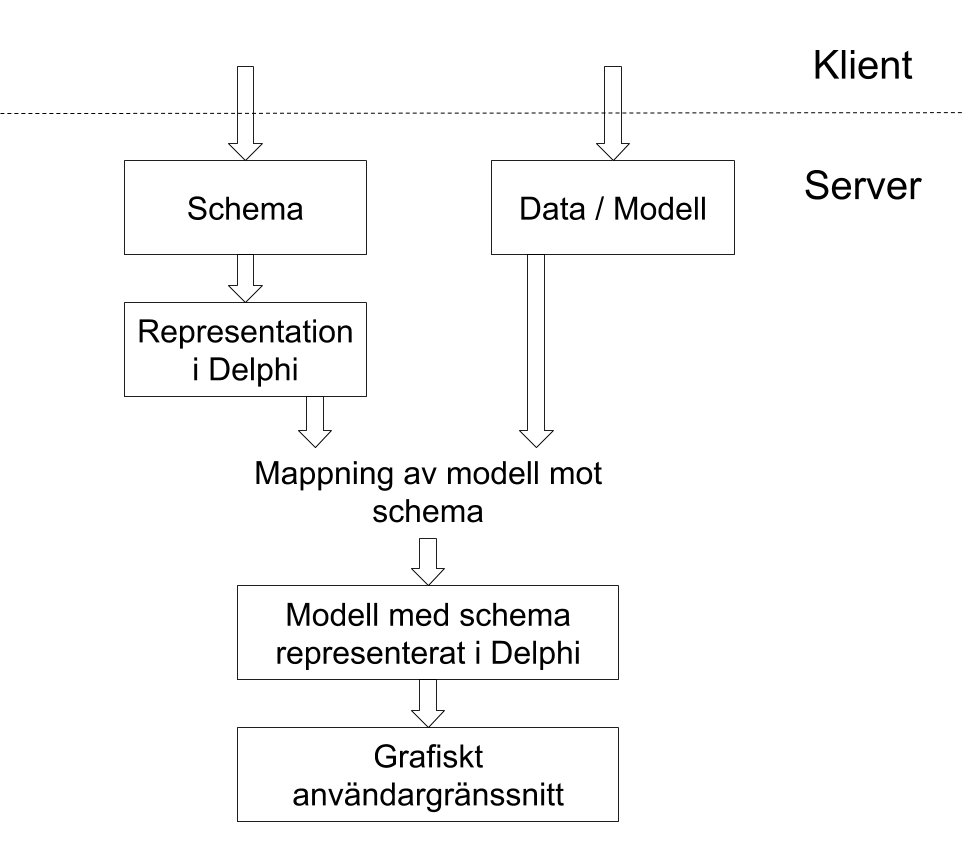
\includegraphics[width=0.9\textwidth,left]{./images/system-ner.png}
		\caption{Flödesschema över systemet}
		\label{fig:system:ner}
	\end{subfigure}
	\begin{subfigure}{0.5\textwidth}
		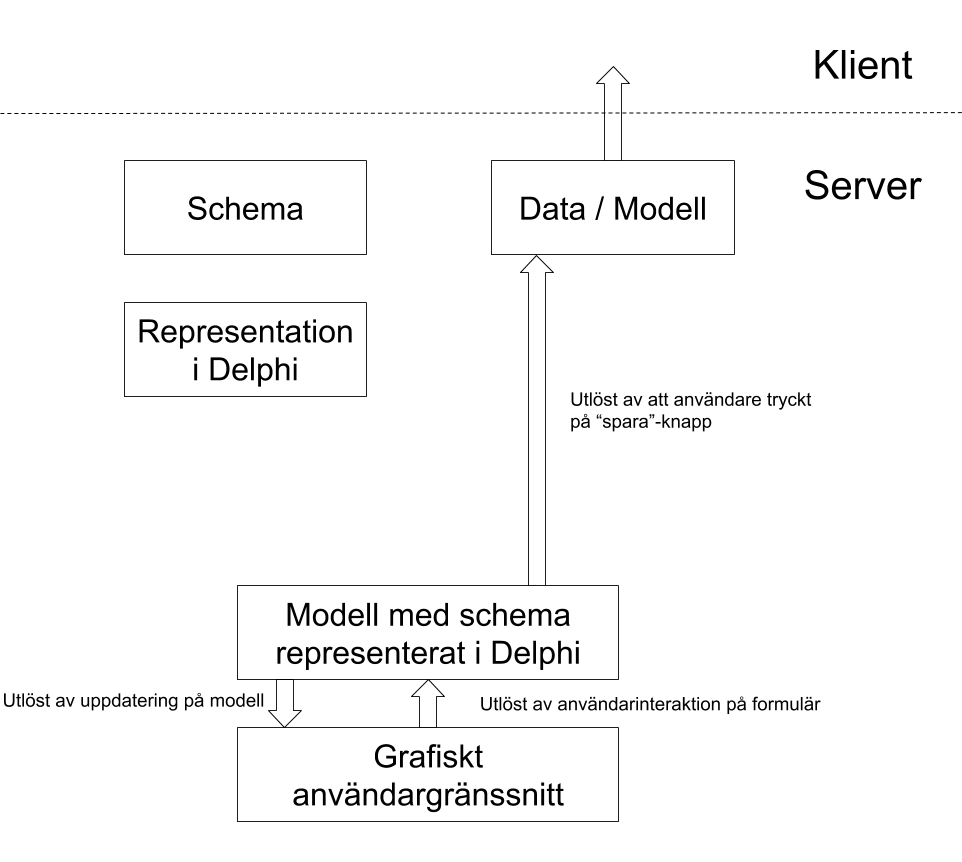
\includegraphics[width=0.9\textwidth,right]{./images/system-upp.png}
		\caption{Flödesschema över systemet}
		\label{fig:system:upp}	
	\end{subfigure}
	\caption{Illustration av dataflöde till och från användargränssnittet}
	\label{fig:system}
\end{figure}

\section{Generering av JSON Schema i Delphi}

Hur JSON Schemat genereras, påverkar inte slutanvändaren, men det påverkar utvecklarna som ska jobba med systemet, och kan hindra vilken funktionalitet som finns tillgänglig i systemet. Ett alternativ är självklart att skriva scheman för hand, men då olika klienter måste ha olika scheman, måste utvecklare se till att rätt schema hamnar på rätt klient vid instalationen av Mimer SoftRadio. Om en kund skulle vilja uppgradera funktionaliteten hos sin installation av Mimer SoftRadio, och därmed behöva tillgång till fler konfigurerbara inställningar i systemet, skulle schemat behöva uppdateras efteråt.

Ett annat alternativ är att basera schemat på inbyggda datatyper i det statiskt typade språket Delphi. Json.NET Schema, NJsonSchema for .NET, typescript-json-schema samt Typson erbjuder exakt den här funktionaliteten i språken .NET respektive TypeScript. För att lägga till extra beskrivningar av datan som språket inte räcker till för, använder .NET-implementationerna \textit{Data Annotation Attributes}, och TypeScript-implementationerna använder experimentella \textit{Decorators}. \cite{Suter,Newtonsoft,El-Dardiry,Bovet} Delphi erbjuder liknande funktionalitet med \textit{Attributes (RTTI)} \cite{Embarcadero2016}. Att annotera datastrukturerna som faktiskt sedan kommer användas i ett system kan automatisera väldigt mycket. Det passar jättebra om det handlar om att bygga ett API där JSON Scheman ska användas för att beskriva för klienter hur och vilken data de kan manipulera. Då kan scheman dynamiskt skapas vid exekvering och de är alltid synkroniserade med datan som systemet är konstruerat för att hantera. Problemet med den lösningen är att schemat i det här arbetet inte ska användas för att beskriva vilken data som kan manipuleras på servern, utan det ska användas för att beskriva hur ett användargränsnitt ska se ut. Den data som ska presenteras på användargränsnittet är en delmängd av all tillgänglig data på servern. Det skulle kunna gå att lägga till annoteringar som beskriver vilken data som ska finnas med på schemat, men det finns enklare lösningar.

Alternativet att handskriva JSON Scheman kräver mycket uppräthållning av scheman och är väldigt mottagligt för misstag hos utvecklarna. Det kräver dock inget system för att dynamiskt generera scheman vid exekvering, då de redan skulle vara genererade. Alternativet att konstruera ett system som använder run-time type information \textit{(RTTI)} är väldigt smidigt för utvecklare under exekvering men kräver relativt mycket utveckling. Ett mellanting skulle vara felsäkert som handskrivna JSON Scheman, men samtidigt dynamiskt genererat vid exekvering för felfria scheman.

JSL är ett exempel på en implementation som erbjuder specifika komplexa datatyper som underlättar genererandet av JSON Scheman. JSL skiljer på datastrukturerna som används för att representera och manipulera data, och själva schemat som används för att beskriva de tidigare nämnda datastrukturerna. \cite{Romanovich} Det ansågs vara ett väldigt praktiskt mellanting. Scheman skrivs för hand men de skrivs inte som JSON Scheman. Istället skrivs de som instanser av komplexa datatyper i Delphi, som sedan under exekvering dynamiskt tolkas för att generera ett JSON Schema. Det här tillåter servern att under exekvering utföra logiska bedömningar för att inkludera exakt det som ska inkluderas i schemat, beroende på vilken version av Mimer SoftRadio operatörsdatorn har, och med vilken tillgänglig funktionalitet datorn har. Schemagenerering är frikopplat från databehandling, men är samtidigt dynamiskt genererat utifrån tillgänglig funktionalitet på operatörsdatorn. Ett exempel på ett genererat schema presenteras i figur \ref{fig:real-schema}.

\begin{figure}
	\inputminted[tabsize=2, frame=single, fontsize=\small, framesep=2mm, breaklines]{json}{code/schema.json}
	\vspace{-1.7em}
	\caption{Exempel på genererat schema}
	\label{fig:real-schema}
\end{figure}

Att generera scheman från JSON-filer ansågs inte vara praktiskt genomförbart (se kapitel \ref{sec:forarbete:json-till-schema}), och skulle inte kunna uppräthålla kraven på systemet. Det skulle dessutom helt ta bort möjligheten för utvecklare att beskriva användargränssnittet.

\section{Parsningen av JSON Schema i Delphi}
\label{sec:arbetet:parsning}

Parsningen av JSON Scheman skedde på ett liknande sett som scheman genererades. För att förenkla arbetet skapades en hjälpklass för att hantera scheman i Delphi. Det innehöll olika objekt \textit{(records)} för att representera olika komponenter i JSON Scheman, samt hjälpfunktioner för att generera JSON Scheman utifrån objekten, och parsa JSON Scheman för att sedan få dessa objekt. Ett tillägg till enkla JSON Scheman var att dessa objekt också kunde innehålla värdet av komponenten den innehöll. Utöver hjälpfunktioner för att parsa och generera scheman fanns bland annat också hjälpfunktioner som användes för att bestämma vilken grafisk komponent som skulle användas för att representera datan.

Strukturen av dessa JSON Scheman kunde antas ha en förutsatt struktur, då användningsområdet var väl känt, samt att både klient och server utvecklades med åtanke till varandra och ingen annan tjänst. Alla inställningsfiler som skulle manipuleras av användargränssnittet hade en liknande struktur som figur \ref{fig:profile-file}. Hela filen är ett objekt, med inställningsgrupper som properties. Figuren har bara en inställningsgrupp men det finns möjlighet för fler. Varje inställningsgrupp är också ett objekt, och den har properties som representerar inställningar. Dessa inställningar är alltid en textsträng, ett heltal, eller ett booleskt värde. Det går därför att utforma parsningen utifrån den här förutbestämda strukturen.

\begin{figure}
	\inputminted[tabsize=2, frame=single, fontsize=\small, framesep=2mm, breaklines]{json}{code/0.json}
	\vspace{-1.7em}
	\caption{Exempel på genererad inställningsfil}
	\label{fig:profile-file}
\end{figure}
\FloatBarrier

\noindent
För att både generering och parsning hanterades av samma tjänst ansågs nyckelordet \textit{definitions} och \textit{\$ref} vara onödigt. Parsern hade därför inte stöd för de två nyckelorden. Det var också känt att parsern aldrig skulle behöva hantera vektorer \textit{(array)} som datatyp vilket innebar att alla nyckelord relaterade till array kunde ignoreras i implementationen. Utöver det var den grundläggande strukturen väl känd och därför behövdes inte nyckelord som:

\begin{itemize}
	\item if
	\item then
	\item else
	\item allOf
	\item anyOf
	\item oneOf
	\item not
\end{itemize}

\noindent
Det fanns fler nyckelord som inte implementerades då bara en delmängd av JSON Schema. För att flersvarsalternativ skulle kunna erbjudas i användargränssnittet implementerades stöd för nyckelordet \textit{enum}, dock med vissa tillägg vilket diskuteras mer i kapitel \ref{sec:arbetet:gui}.

Figur \ref{fig:system:ner} beskriver systemet i helhet och där är parsningen en viktig del av dataflödet. Först parsas schemat för att skapa en representation av schemat i Delphi, med de tidigare nämnda objekten. Objekten innehåller också värdet av datan de beskriver men i det första steget är alla värden tomma. Nästa steg är att traversera JSON-filen som innehåller den riktiga datan, och sedan populera objekten med korrekta värden. Först då kan användargränssnittet genereras.

\section{Representation av data i användargänssnittet}
\label{sec:arbetet:gui}

Många implementationer diskuterade i \ref{sec:forarbete:gui-generering} använder ett extra JSON-dokument för att beskriva hur schemat, och modellen schemat representerar ska presenteras i användargränssnittet. Det ansågs vara överflödigt att behöva skicka två dokument som båda ska användas vid exakt samma steg i systemet. Det andra alternativet för att utöka funktionalitet hos JSON Schema är att använda egna nyckelord i schemat som inte finns standardiserade i JSON Schema specifikationerna. Det här arbetet krävde nästan ingen utökad funktionalitet hos JSON Scheman, förutom förbättrad funktionalitet hos \textit{enum} vilket diskuteras mer i kapitel \ref{sec:arbetet:gui:enum}. Det gick att generalisera användargränssnittet tillräckligt för att hantera alla datatyper som systemet använder sig av, och presentera ett relevant användargränssnitt av dem. Nyckelordet \textit{format} kunde erbjuda väldigt hög kontroll av användargränssnittet.

\subsection{Det generella användargränssnittet}

Det enklaste valet av grafiskt användargränssnitt skulle vara att erbjuda en generell JSON editor där datan visuellt representeras med en trädstruktur. Det finns många exempel på användargränssnitt som erbjuder ett grundläggande gränssnitt för att redigera generell JSON-data. De skiljer sig inte mycket mot att skriva JSON manuellt, men kan erbjuda enkel hjälp med nyckelord och formatering. Figur \ref{fig:json-editor} visar JSON Editor Online, vilket är ett exempel på ett sådant användargränssnitt \cite{DeJong2018}. Det skulle behöva begränsa vad användaren skulle kunna mata in med hjälp av JSON Schemat men ett sådant formulär har möjlighet att hantera JSON Data som följer all möjlig sorts struktur. Det vore en stor fördel att kunna erbjuda ett formulär som kan hantera alla möjliga sorters scheman. En nackdel med att använda ett sådant användargränssnitt är att det inte är särskillt anpassat för ändamålet, och gränssnittet blir inte särskillt frikopplat mot datan som ska manipuleras. Det blir dessutom svårt att presentera information till användaren som kan hjälpa användaren förstå hur datan kommer användas.

\begin{figure}
	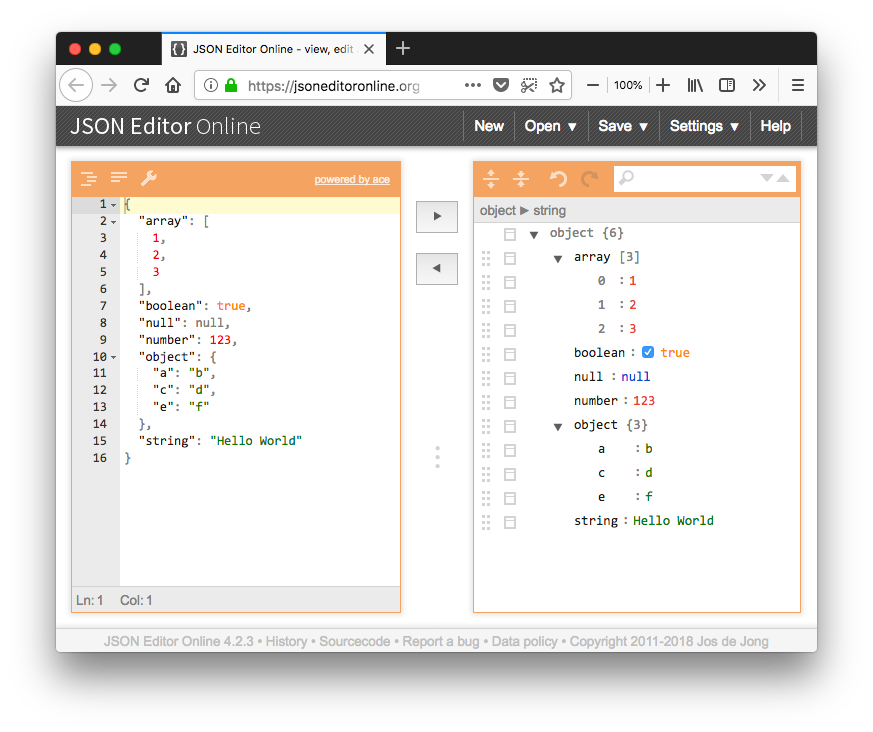
\includegraphics[width=\textwidth]{./images/screenshot-json-editor.png}
	\vspace{-1.7em}
	\caption{JSON Editor Online \cite{DeJong2018}}
	\label{fig:json-editor}
\end{figure}

Ett annat alternativ är att göra som React JSON Schema Form (se figur \ref{fig:react-jsonschema-form}). React JSON Schema Form genererar ett webbformulär utifrån ett JSON Schema och ett extra JSON-dokument som kallas UISchema \cite{MozillaServices}. Varje datanod som kan manipuleras representeras med ett inmatningsfält och objekt och vektorer representeras med visuella grupperingar. Användargränssnittet blir mycket mer anpassat till syftet, och lättare att använda. Dessutom utnyttjas annoteringsnyckelorden \textit{title} och \textit{description} från JSON Schemat, för att förklara för användaren vad datan betyder. Det som kan bli svårt med en design som är anpassad efter syftet som ett formulär är hur komplexa JSON-strukturer ska hanteras. Hur skulle exempelvis en vektor innehållande objekt med två properties, varav ena propertyn är ett objekt med två olika vektorer, presenteras på ett användarvänligt sätt? Att även presentera annoteringar som \textit{title} och \textit{description} till alla datanoder i det formuläret vore ännu en till utmaning. En vanlig JSON-Editor klarar av att presentera djupt komplexa datatyper, medan det kan vara väldigt svårt att göra samma sak på ett generellt sätt med formulär. Många lösningar som React JSON Schema Form erbjuder generella formulär som klarar av alla JSON Scheman, med alternativet att specificera mer hur formuläret ska se ut, med hjälp av ett extra JSON-dokument. \cite{MozillaServices} Det är en riktigt bra kompromiss om lösningen måste kunna klara av att presentera djupt komplexa datatyper, som inte följer en förutbestämd struktur.

\begin{figure}
	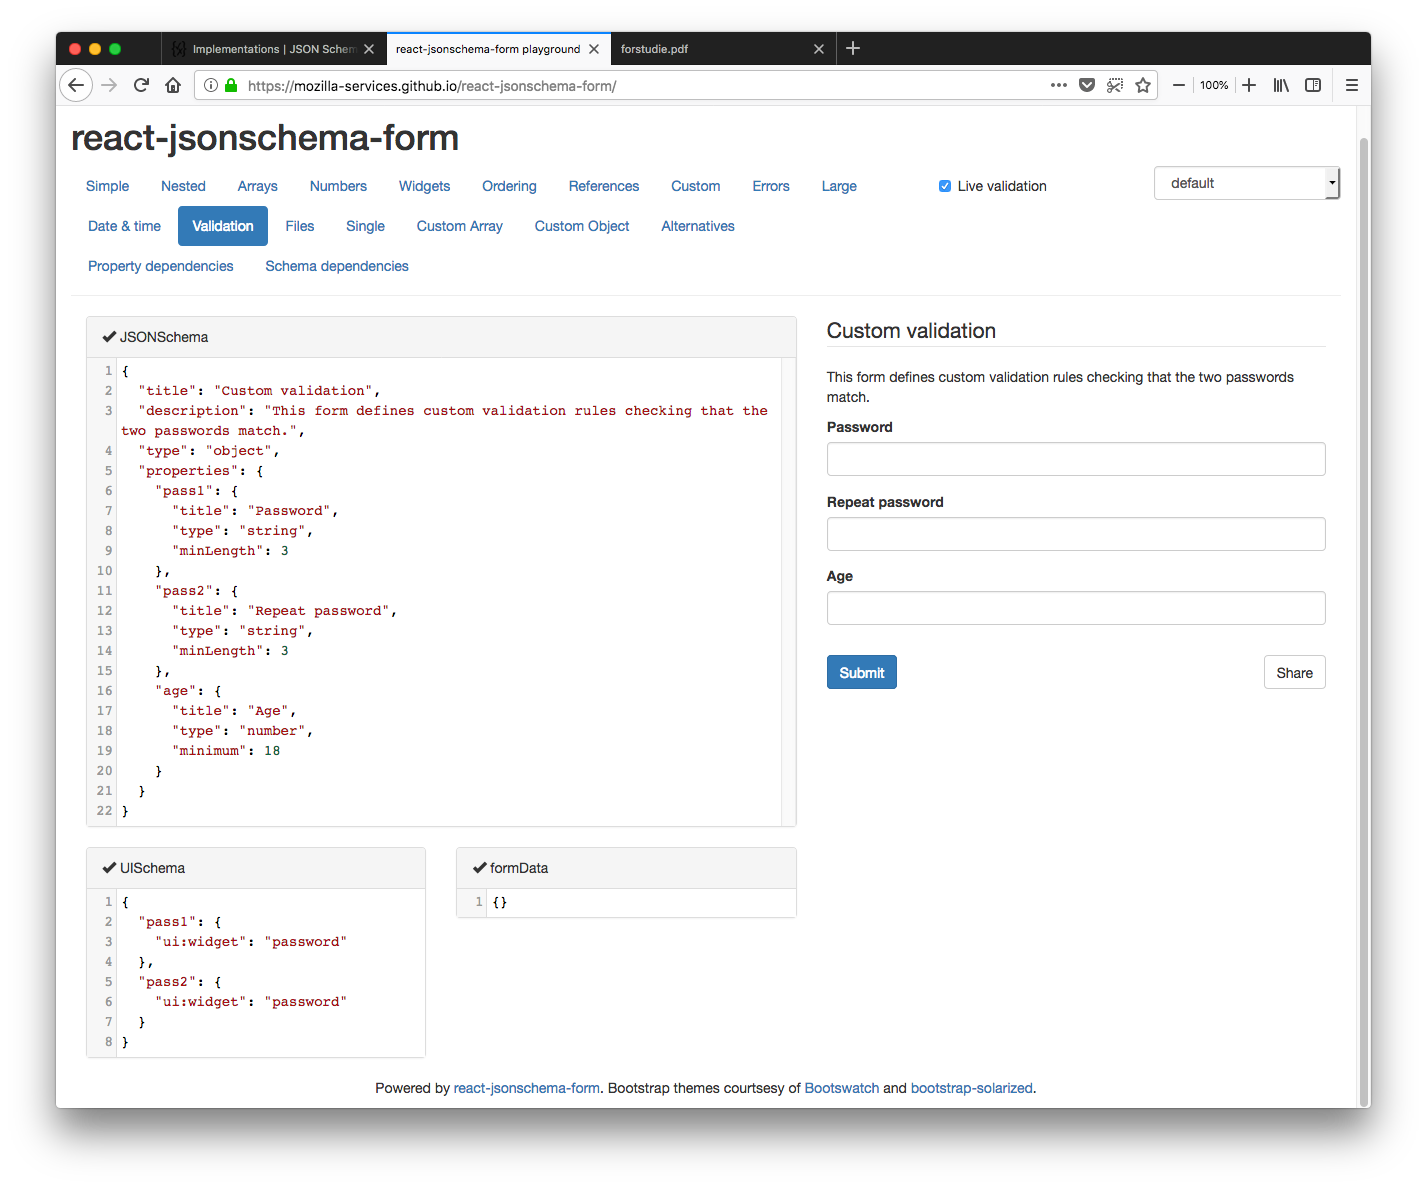
\includegraphics[width=\textwidth]{./images/screenshot-react-jsonschema-form.png}
	\vspace{-1.7em}
	\caption{React JSON Schema Form \cite{MozillaServices}}
	\label{fig:react-jsonschema-form}
\end{figure}

Datan som skulle presenteras på användargränssnittet i arbetet var varken komplex eller totalt generell. Datan bestod av ett objekt med flera objekt som properties, där de objekten i sin tur var antingen en textsträng, ett heltal eller ett booleskt värde. Datan var som mest tre lager djup. Det gick dessutom att dela in datanoderna i inställningsgrupper och inställningsnoder. Därför kunde både en JSON-editor användas, eller ett formulär. Datan som skulle presenteras ansågs av LSE vara för komplex för många användare att förstå utan en ordentlig förklaring av varje inställningsnod. Däremot ansågs inte ett enda formulär ge tillräcklig överblick över alla inställningar och skulle inte utnyttja grupperingen av inställningar. JSON-typerna \textit{string}, \textit{number}, \textit{integer} och \textit{boolean} ansågs tjäna på att representeras i ett platt formulär medan typerna \textit{object} och \textit{array} tjänade på att representeras i en trädstruktur. Det bästa alternativet ansågs därför vara att kombinera de två ovanstående representationerna. Användargränssnittet presenteras i figur \ref{fig:gui:helhet}.


\begin{figure}
	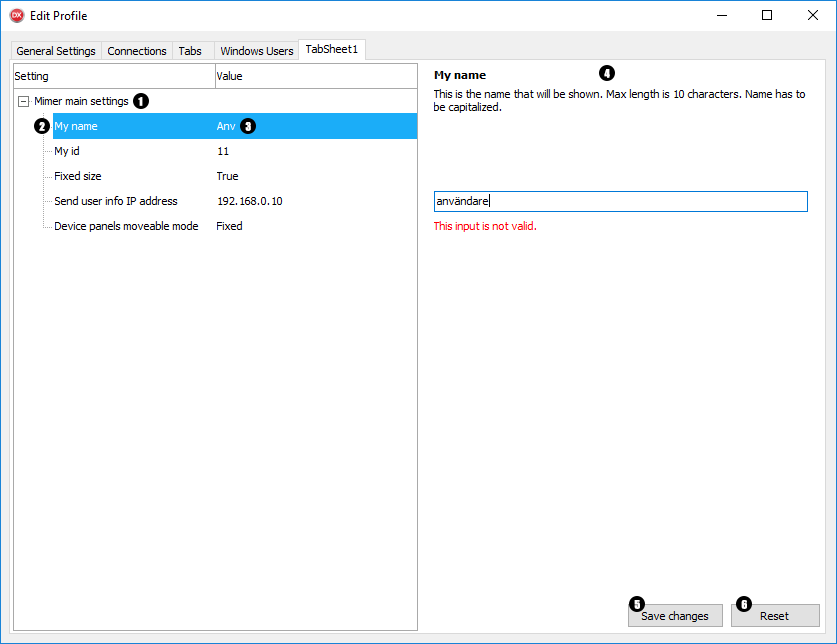
\includegraphics[width=\textwidth]{./images/gui/helhet-copy.png}
	\vspace{-1.7em}
	\caption{Användargränssnittet av administratörsprogrammet \textbf{(TODO! ta ny bild!!!)}}
	\label{fig:gui:helhet}
	\begin{enumerate}
		\item Inställningsgrupp
		\item Namn på inställning
		\item Värde på inställning
		\item Formulär för att ställa in inställning
		\item Spara-knapp
		\item Omstarts-knapp
	\end{enumerate}
\end{figure}

Ena halvan av det grafiska användargränssnittet användes en trädstruktur för att presentera presentera tillgängliga inställningar och inställningsgrupper, eller mer generellt representerades JSON-objekt och dess tillgängligga \textit{properties}. Det skulle kunna gå att lägga till grafiska interaktionselement för att erbjuda användaren att lägga och ta bort \textit{properties} från objekt eller element från vektorer, men det JSON-filerna som skulle manipuleras hade bestämd struktur på sina \textit{properties} och vektorer skulle inte hanteras.

Den vänstra halvan tillät inte användaren att manipulera någon \textit{property} (inställning) utan bara välja den. Andra halvan av användargränssnittet användes för att presentera den valda inställningen, med beskrivning av inställningen samt möjligheter att ändra värdet på den valda inställningen. Beslutet grundades på att det skulle vara enkelt för användaren att få en överblick över vilka inställningar som fanns tillgängliga, samtidigt som varje inställning skulle vara enkel att förstå och ändra. Värdena på inställningarna kan alltid synas utan att en inställning väljs men en inställning måste väljas för att kunna bli manipulerad. Namnet på inställningsgrupperna och inställningarna är frikopplade från deras riktiga namn data-filerna och modellen med hjälp av nyckelordet \textit{title} i JSON Schemat.

För att förenkla för användaren erbjuds en omstarts-knapp som raderar alla osparade ändringar och startar om formuläret så att formuläret motsvarar inställningarna på servern. Vid varje användarinteraktion, där en användare manipulerar ett värde på formuläret, propageras ändringen till datamodellen vilket i sin tur uppdaterar hela användargränsnittet, men ändringen skickas inte till servern. Användaren har erbjudits en spara-knapp och först då förmedlas alla ändringar till servern. Då användargränssnittet skulle användas både för data med delvis förutbestämd struktur och inte djupt komplex data ansågs ett extra JSON-dokument för att lägga till extra specificering av användargränsnittet överflödigt och onödigt komplext.

Användargränssnittet som utvecklades blev tvådelat, där ena halvan av gränssnittet användes för att presentera tillgängliga inställningar och inställningsgrupper, samt låta användaren välja en inställning att manipulera. Andra halvan av användargränssnittet användes för att presentera en inställning, med beskrivning av inställningen samt möjligheter att ändra värdet på den valda inställningen. Beslutet grundades på att det skulle vara enkelt för användaren att få en överblick över vilka inställningar som fanns tillgängliga, samtidigt som varje inställning skulle vara enkel att förstå och ändra. Värdena på inställningarna kan alltid synas utan att en inställning väljs men en inställning måste väljas för att kunna bli manipulerad. Namnet på inställningsgrupperna och inställningarna är frikopplade från deras riktiga namn data-filerna och modellen med hjälp av nyckelordet \textit{title} i JSON Schemat.

För att förenkla för användaren erbjuds en omstarts-knapp som raderar alla osparade ändringar och startar om formuläret så att formuläret motsvarar inställningarna på servern. Vid varje användarinteraktion, där en användare manipulerar ett värde på formuläret, propageras ändringen till datamodellen vilket i sin tur uppdaterar hela användargränsnittet, men ändringen skickas inte till servern. Användaren har erbjudits en spara-knapp och först då förmedlas alla ändringar till servern.

\subsection{Hur formuläret förhindrar fel}

Syftet med JSON-scheman är till stor del att förhindra att inkompatibel data sparas och används i applikationer. Det kan handla om att ett användargränssnitt inte är byggt för att presentera viss sorts data, eller att ett helt system upphör att fungera för att systemet inte kunde hantera den sparade datan. Användningen av JSON Scheman i det här arbetet handlar också om att säkerställa att enbart kompatibel data skickas mellan klient och server. En kritisk frågeställning vid utvecklandet av ett intuitivt användargränsnitt är hur felaktiga användarinteraktioner ska hanteras i användargränssnittet.

Den enklaste hanteringen av inkompatibel data, är att när en användare har givit inkompatibel data, kan ett generiskt felmeddelande presenteras, samt att användaren förhindras från att spara datan före användaren givit kompatibel data. Det förlitar sig på att varje inställning har en tillräckligt utförlig förklaring för hur datan ska formateras. Ett annat alternativ är att förhindra att användaren kan mata in felaktig data. Det kan exempelvis handla om att användaren bara kan mata in siffror till formuläret, om datan ska formateras som en siffra. Om användaren försöker mata in en bokstav så ignoreras den användarinteraktionen. Det kan kompleteras med förklaringar av korrekt formatering i inställningsbeskrivningen, men att användaren inte ens kan mata in inkompatibel data är väldigt intuitivt. Det perfekta målet vore att när en användare matar in inkompatibel data, ändrar formuläret datan till den närmsta kompatibla datan. Om en användare matar in siffran 300 i ett formulär som bara tillåter siffror upp till siffran 255 så kan formuläret automatiskt ändra värdet till 255. Det kan dock vara svårt att lösa för mer komplexa situationer.

För att erbjuda en grundlägande användbarhet av formuläret presenterades olika sorters inmatningsfält beroende på om typen av inställning var en textsträng, en siffra eller ett booleskt värde. Detta förhindrade att användare kunde mata in data som var av fel typ. Det fanns fler fall där ännu fler olika inmatningsfällt kunde presenteras beroende på mer formateringsinformation av datan. När det gick så skapades formuläret så att den aldrig tillät användaren att mata in inkompatibel data, men i vissa fall visades bara ett felmeddelande. Hur olika formateringar specificerat i schemat uppräthölls beskrivs i resten av kapitlet.

\subsection{Textsträngar och \textit{format} i användargränssnittet}

När en vald inställning ska vara formaterad som en sträng, presenteras ett inmatningsfält för strängar, som i figur \ref{fig:textstrang}. JSON Schema erbjuder tre valideringsnyckelord enbart för textsträngar: \textit{maxLength}, \textit{minLength} samt \textit{pattern}. Nyckelorden \textit{maxLength} och \textit{minLength} används för att bestämma längden av textsträngen. Nyckelordet \textit{pattern} bestämmer att textsträngen måste följa ett mönster, som specificeras som ett regular expression enligt ECMA 262 regular expression dialect \cite{EcmaInternational2017}. Utöver de tre nyckelorden finns det ett fjärde nyckelord som är applicerbart på textsträngar, vilket är \textit{format}. I de senaste JSON Schema specifikationerna är samtliga åtta definerade format enbart applicerbara på textsträngar. Det går att applicera nyckelordet \textit{format} på vilken datatyp som helst, vilket kort kommer diskuteras senare i rapporten. \cite{Andrews}

\begin{figure}
	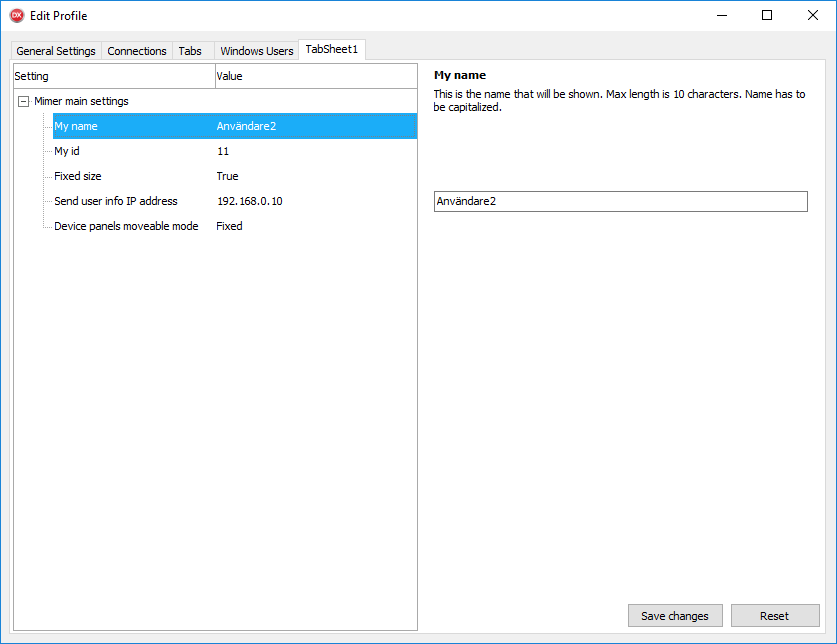
\includegraphics[width=\textwidth]{./images/gui/textstrang.png}
	\vspace{-1.7em}
	\caption{Inmatningsfält för textsträngar}
	\label{fig:textstrang}
\end{figure}

Om en användare försöker mata in en karaktär i inmatningsfältet, och textsträngen redan är lika lång som den maximala tillåtna längden, ignoreras användarinteraktionen. På det sättet går det inte ens för en användare att mata in inkompatibel data, och försöka förstå hur korrekt formaterad data ska se ut. Detta bör kompleteras med en förklaring i beskrivningen av inställningen, så att användaren förstår varför formuläret hanterar användarinteraktioner på det sättet.

Om en användare försöker ta bort så många karraktärer så att textsträngens längd är kortare än den minsta tillåtna längden, presenteras ett felmeddelande och den senaste tillåtna datan sparas i modellen (se figur \ref{fig:textstrang-minLength}). Det skulle kunna gå att förhindra användaren från att ta bort så många karraktärer, men det skulle kunna upplevas som omständigt av användaren, då det kan finnas fall då användaren vill ta bort hela textsträngen för att byta ut textsträngen mot en helt ny. Om användaren skulle förhindras från att ta bort för många karraktärer, och användaren skulle vilja byta ut hela textsträngen mot en helt annan, skulle användaren behöva mata in den nya samtidigt som den gamla delvis var kvar, vilket inte ansågs vara användarvänligt. Att kombinera det med en maximal längd på textsträngar skulle tvinga användaren att hela tiden förhålla sig inom ett intervall av textsträngslängd.

\begin{figure}
	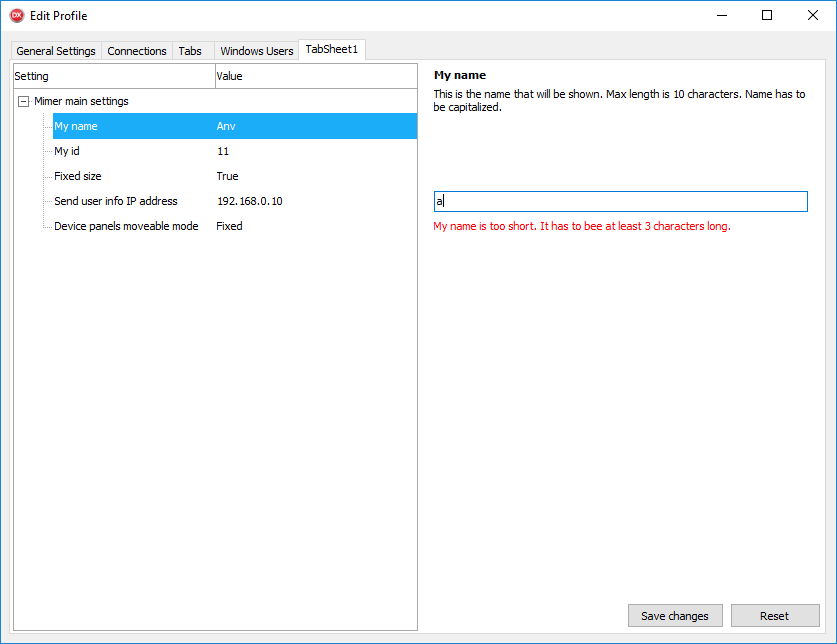
\includegraphics[width=\textwidth]{./images/gui/textstrang-minLength.png}
	\vspace{-1.7em}
	\caption{Felmeddelande vid för kort textsträng}
	\label{fig:textstrang-minLength}
\end{figure}

Om formatet av textsträngen är mer komplext än längd kan \textit{pattern} användas för att specificera väldigt komplexa mönster som en textsträng måste upprätthålla. Det kan exempelvis användas för att specificera att en textsträng ska inledas med versal som i figur \ref{fig:textstrang-pattern}. Då regular expression-mönster kan vara väldigt komplexa och oförutsägbara, är det svårt att hitta ett närmsta kompatiblet värde. Därför presenteras ett felmeddelande när textsträngen inte följer mönstret. Då det inte går att veta hur mönstret fungerar på ett användarvänligt sätt, används ett generiskt felmeddelande, vilket innebär att det är viktigt att inställningsbeskrivningen beskriver formatet som textsträngen ska följa.

\begin{figure}
	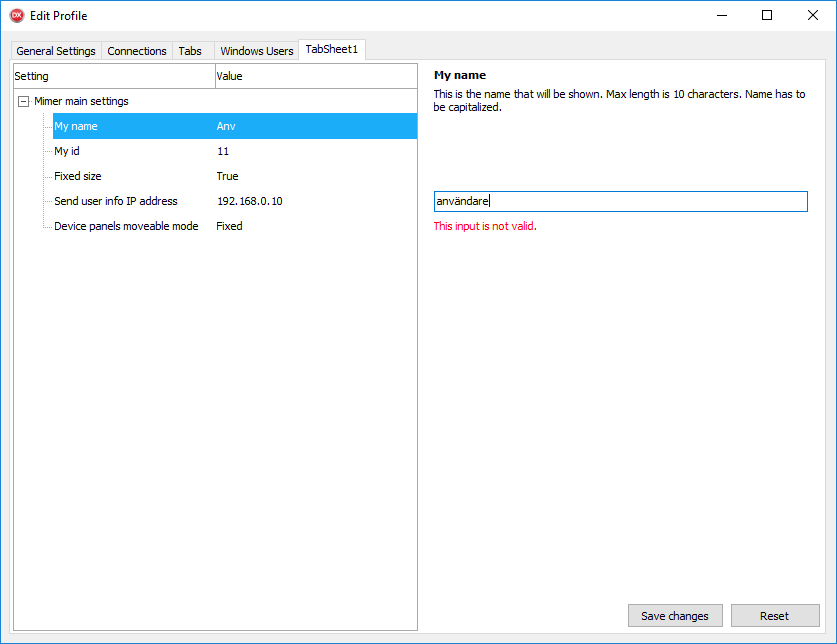
\includegraphics[width=\textwidth]{./images/gui/textstrang-pattern.png}
	\vspace{-1.7em}
	\caption{Felmeddelande vid för textsträng som inte följer regular expression-mönstret}
	\label{fig:textstrang-pattern}
\end{figure}

\FloatBarrier
\subsection{Nyckelordet \textit{format}}

Nyckelordet \textit{pattern} är jättebra för att säkerställa att textsträngar följer ett mer komplext format än enbart längden på textsträngen, men \textit{pattern} kan inte användas för att bestämma hur inmatningsfältet ska se ut. Ibland skulle det passa bättre att presentera ett inmatningsfält som är mer lämpat för en specifik textsträng. Det kan exempelvis passa med ett litet inmatningsfält för korta textsträngar som bara ska vara ett eller några ord, men vid längre texter kanske ett större inmatingsfält behövs. Nyckelordet \textit{format} används både för annotering och validering enligt JSON Schema specifikationerna och får användas för att beskriva egna format på JSON-värden, som inte nödvändigtvis måste följa en standard upprättad av IETF, men som måste vara förutbestämd av alla parter i samma system \cite{Andrews2018}.

För validering kan \textit{format} användas när nyckelordet \textit{pattern} inte räcker, eller blir komplext att använda, och för annotering kan det användas för att förklara formatet av ett JSON-värde. Det kan också användas för att annotera för ett användargränssnitt, att ett JSON-värde borde presenteras på ett specifikt sätt. Figur \ref{fig:textstrang-ip-format} visar hur \textit{format} används för att beskriva att en textsträng ska vara formaterad som en IPv4-adress. I det fallet kan ett specifikt inmatningsfält erbjudas, som bara tillåter användaren att mata in en IPv4-formaterad textsträng.

Nyckelordet \textit{format} kan användas för andra typer än textsträngar och systemet som utvecklas har stöd både på klienten och servern, för att använda \textit{format} till siffror och booleska värden. När \textit{format} används till textsträngar är det viktigt att poängtera att det borde kompleteras med \textit{pattern} om möjligt. Alla delar av systemet ska vara bakåtkompatibla med tidigare versioner av systemet, för en betydligt lång tidsperiod, och om nya sorters \textit{format} läggs till, kan vissa äldre instanser av klienter vara inkompatibla med den sortens \textit{format}.

\begin{figure}
	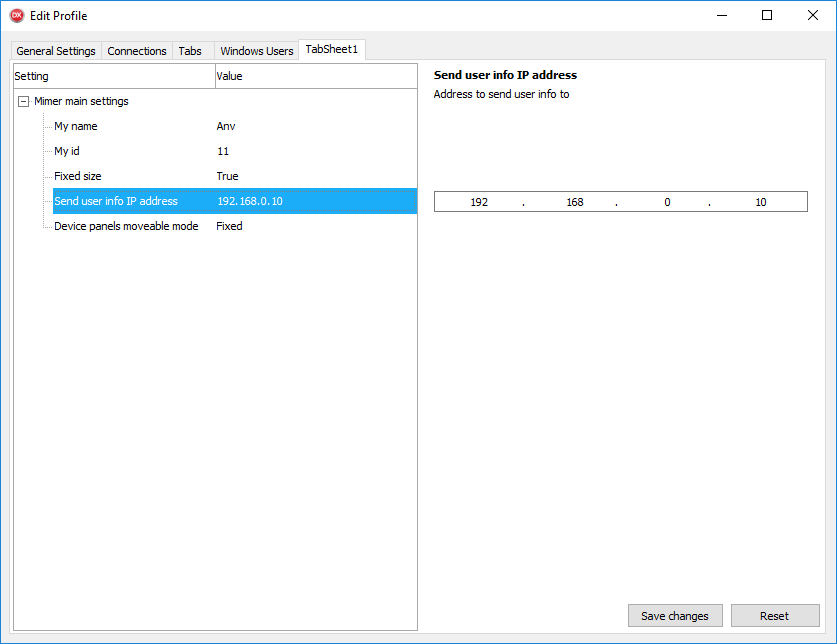
\includegraphics[width=\textwidth]{./images/gui/textstrang-ip.png}
	\vspace{-1.7em}
	\caption{Textsträng formaterad som en IPv4-adress}
	\label{fig:textstrang-ip-format}
\end{figure}


\FloatBarrier
\subsection{Booleska värden och heltal i användargränssnittet}

Booleska värden kan bara vara ett av två värden. Inmatningsfältet som valdes för att presentera booleska värden blev en kryssruta, som visas i figur \ref{fig:bool}. Det finns ingen möjlighet för användaren att mata in ett annat värde än de två tillåtna värdena. Om användargränssnittet ska presentera något annat värde än \textit{true} eller \textit{false} kan nyckelordet \textit{enum} användas, vilket diskuteras mer senare.

\begin{figure}
	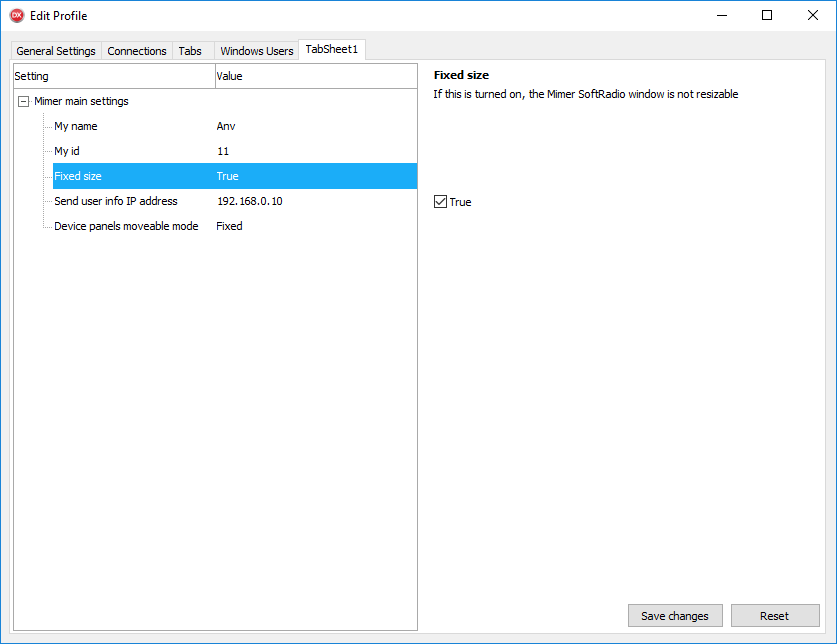
\includegraphics[width=\textwidth]{./images/gui/bool.png}
	\vspace{-1.7em}
	\caption{Kryssruta för ett booleskt värde}
	\label{fig:bool}
\end{figure}

Utöver booleska värden och textsträngar skulle systemet klara av att hantera heltal. Då hanteringen av flyttal fortfarande ansågs vara experimentel och ofärdig, samt att det saknades behov av flyttal så implementerades bara stöd för heltal. Då både klient och server utvecklades med hänsyn till varandra, i samma språk (Delphi), samt att systemet inte var byggt för att hantera flyttal, kunde alla siffror antas vara heltal, och inga oklarheter kring vad som räknas som heltal (se kapitel \ref{sec:teori:schema:float}) behövde hanteras. Om något tal skulle skickas som ett flyttal skulle det talet avrundas och hanteras som ett heltal vid parsningen av JSON-filen.

Heltal presenterades som i figur \ref{fig:heltal}. Inmatningsfältet hanterar endast siffror och har dessutom två hjälpknappar för att höja och sänka värdet i steg. Det finns fem valideringsnyckelord enbart för siffror: \textit{multipleOf}, \textit{maximum}, \textit{exclusiveMaximum}, \textit{minimum} samt \textit{exclusiveMinimum}. Nyckelordet \textit{multipleOf} kräver att siffran som valideras ska vara jämnt delbart med värdet beskrivet av \textit{multipleOf}. Användningsområdet för \textit{multipleOf} ansågs inte vara applicerbart för systemet och därför ignorerades. De resterande fyra nyckelorden specificerar ett interval som siffran måste befinna inom. Om en användare försökte mata in ett värde som var utanför intervallet så ändrades värdet till det närmaste kompatibla värdet inom intervallet. \cite{Andrews2018}

\begin{figure}
	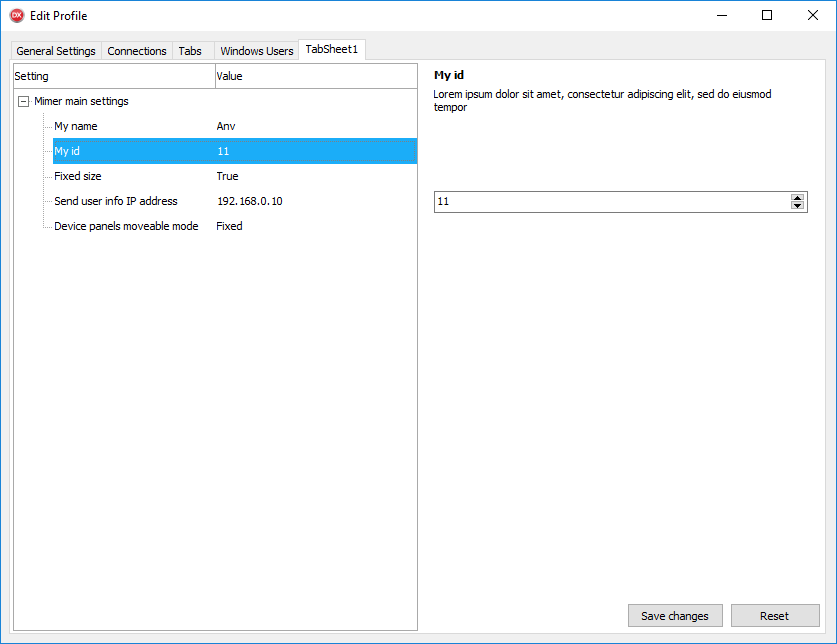
\includegraphics[width=\textwidth]{./images/gui/heltal.png}
	\vspace{-1.7em}
	\caption{Inmatningsfält för heltal}
	\label{fig:heltal}
\end{figure}

Om stöd för flyttal skulle behövas i framtiden, föreslås att nyckelordet \textit{format} används för att specificera det. Det skulle kunna hanteras på ett sätt som är bakåtkompatibelt med klienter som bara kan hantera heltal, genom att de klienterna hanterar flyttalen som heltal, samtidigt som nyare klienter kan hantera flyttalen som flyttal.

\FloatBarrier
\subsection{Flervalsalternativ och \textit{enum} i användargränssnittet}
\label{sec:arbetet:gui:enum}

Vissa inställningar hade så pass begränsade tillåtna alternativ att bara ett fåtal alternativ på värden var tillåtna. Då användes nyckelordet \textit{enum}. Nyckelordet \textit{enum} används för att specificera en lista med tillåtna värden. Inmatningsfältet som valdes var en lista med alternativ som användaren kan välja, som presenteras i figur \ref{fig:enum}. Det fanns aldrig fall då olika alternativ skulle vara av olika typer, trots att JSON Schema tillåter det \cite{Andrews2018}.

\begin{figure}
	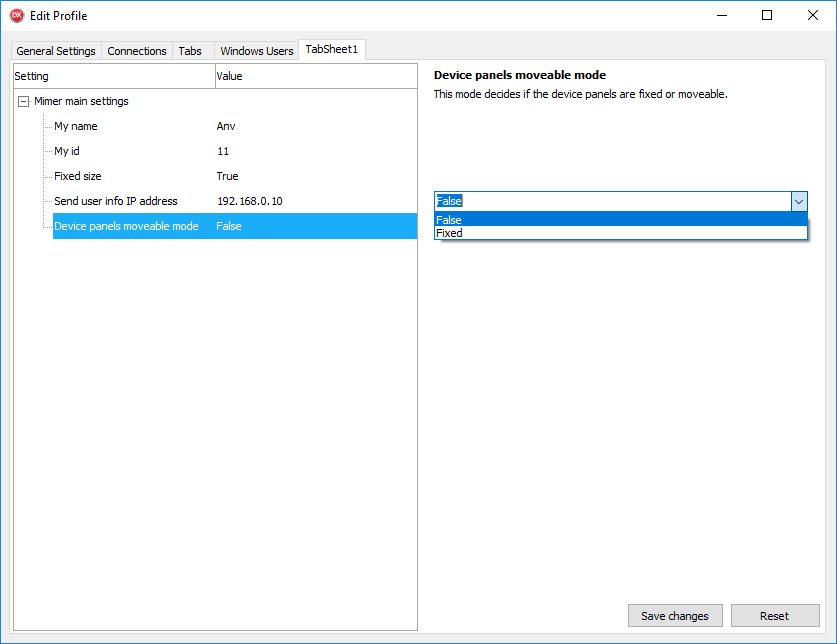
\includegraphics[width=\textwidth]{./images/gui/enum.png}
	\vspace{-1.7em}
	\caption{Inmatningsfält för \textit{enum}}
	\label{fig:enum}
\end{figure}

Enum tillåter inga alternativ för att annotera de förutsatta värdena med metadatainformation som \textit{title} eller \textit{description}. Det innebär att värdena som \textit{enum} specificerar, inte går att koppla till någon annan representation än det faktiska värdet. Ett problem skulle exempelvis kunna uppstå om ett värde bara få ha värdena \textit{1}, \textit{2} eller \textit{3} i en JSON-fil, men användarna ska presenteras med \textit{one}, \textit{two} och \textit{three} som svarsalternativ. React JSON Schema Form bemöter det problemet med att utöka JSON Schema och lägga till nyckelordet \textit{enumNames} som i figur \ref{fig:enum-example:extra-array} \cite{MozillaServices}. Användandet av det nyckelordet är inkompatibelt med JSON Schema \cite{Andrews2018}. Dessutom finns det massor av oklarheter över hur fall skulle hanteras om \textit{enumNames} finns men \textit{enum} saknas, eller om \textit{enumNames} och \textit{enum} innehåller olika antal element.

Ett annat förslag som React JSON Schema Form föreslår är användandet av nyckelordet \textit{anyOf}, vilket är helt kompatibelt med JSON Schema specifikationerna men är väldigt verbost och använder \textit{anyOf} på ett sätt som det inte ursprungligen är menat för att användas på \cite{MozillaServices, Andrews2018}. Dessutom kräver deras implementation att nyckelordet \textit{enum} ska användas för att definera listor innehållande ett konstant värde, vilket inte är syftet med \textit{enum} \cite{Andrews2018}. Deras förslag visas i figur \ref{fig:enum-example:any-of}. Jag föreslår användandet av nyckelordet \textit{const} istället, vilket visas i figur \ref{fig:enum-example:any-of-const}. Nyckelordet är till för att specificera att en definition bara får ha ett enda konstant värde och är mindre än ett år gammalt, vilket kan vara en anledning till att React JSON Schema Form inte användt \textit{const} i sin implementation \cite{Andrews2018}.

\begin{figure}
	\begin{subfigure}[t]{\textwidth}
		\inputminted[tabsize=2, frame=single, fontsize=\small, framesep=2mm, breaklines]{json}{code/enum-example/extra-array.json}
		\vspace{-1.2em}
		\caption{Hur React JSON Schema Form föreslår \textit{enumNames} \cite{MozillaServices}}
		\label{fig:enum-example:extra-array}
		\vspace{.8em}
	\end{subfigure}
	\begin{subfigure}[t]{0.47\textwidth}
		\inputminted[tabsize=2, frame=single, fontsize=\small, framesep=2mm, breaklines]{json}{code/enum-example/any-of.json}
		\vspace{-1.2em}
		\caption{React JSON Schema Forms JSON Schema-kompatibla alternativ till \textit{enumNames} \cite{MozillaServices}}
		\label{fig:enum-example:any-of}
	\end{subfigure}\hfill
	\begin{subfigure}[t]{0.47\textwidth}
		\inputminted[tabsize=2, frame=single, fontsize=\small, framesep=2mm, breaklines]{json}{code/enum-example/any-of-const.json}
		\vspace{-1.2em}
		\caption{Ett modernare förslag av React JSON Schema Forms JSON Schema-kompatibla förslag med \textit{const}}
		\label{fig:enum-example:any-of-const}
	\end{subfigure}
	\caption{Olika alternativ av annotering av \textit{enum}}
	\label{fig:enum-example:any-of-examples}
\end{figure}

Lösningen att använda \textit{anyOf} är helt kompatibelt med JSON Schema men kan introducera många risker för fel, då \textit{anyOf} kan användas för att definera flera olika generella definitioner, vilket är mycket mer komplext än att använda \textit{enum} för förbestämda värden. Jag föreslår ett fjärde alternativ vilket varken introducerar fler nyckelord, eller förlitar sig på att olika nyckelord förhåller sig korrekt till varandra, men som inte är helt kompatibelt med de nuvarande JSON Schema specifikationerna. Jag föreslår att \textit{enum} används som tidigare för att specificera förutbestämda värden, men att ett värde också kan vara ett objekt med vissa bestämda nyckelord som används för annotering. Figur \ref{fig:enum-example:const} är ett exempel på det formatet. Nyckelorden \textit{title}, \textit{description} och \textit{const} skulle kunna reserveras. Ett problem vore hur en parser skulle kunna skilja på ett objekt som faktiskt innehåller en \textit{property} med namnet \textit{title}, men det skulle kunna vara bestämt att om ett element i listan i \textit{enum} innehåller en \textit{const-property} så kommer eventuella \textit{title} och \textit{description} användas som metadata för värdet i \textit{const}. Om ett objekt med en \textit{property} med namnet \textit{title} ska specificeras i \textit{enum} så räcker det med att placera det objektet i ett objekt under dess \textit{const-property} som i figur \ref{fig:enum-example:title}. Självklart går det dessutom att blanda element som bara är värdet de representerar med annoterade objekt. Arbetet använde den här metoden för att hantera \textit{enums} och flervalsalternativ.

\begin{figure}
	\begin{subfigure}[t]{0.47\textwidth}
		\inputminted[tabsize=2, frame=single, fontsize=\small, framesep=2mm, breaklines]{json}{code/enum-example/const.json}
		\vspace{-1.2em}
		\caption{Enkelt förslag på utökning av enum}
		\label{fig:enum-example:const}
	\end{subfigure}\hfill
	\begin{subfigure}[t]{0.47\textwidth}
		\inputminted[tabsize=2, frame=single, fontsize=\small, framesep=2mm, breaklines]{json}{code/enum-example/nested.json}
		\vspace{-1.2em}
		\caption{Förslag på utökning av enum med objekt som använder \textit{title}}
		\label{fig:enum-example:title}
	\end{subfigure}
	\caption{Förslag på utökning av \textit{enums} i JSON Scheman}
\end{figure}
\chapter{Diskussion, slutsats och fortsatt arbete}
\label{sec:slutsats}

Arbetet har utförligt utvärderat JSON Schema, hur grafiska användargränssnitt kan genereras från scheman samt vad som saknas i JSON Scheman. Kapitel \ref{sec:slutsats:json-schema} diskuterar problemen som fortfarande finns med att använda JSON Scheman till att generera grafiska användargränssnitt. Kapitel \ref{sec:slutsats:fortsatt-arbete} föreslår framtida fokusområden att fortsätta arbetet med. Kapitel \ref{sec:slutsats:slutsats} diskuterar arbetet och resultatet av det, samt vilka slutsatser som kan dras efter arbetet.


\section{Att använda JSON Schema för att generera grafiska användargränssnitt}
\label{sec:slutsats:json-schema}
JSON Schema är huvudsakligen ämnat för att validera data, trots att det erbjuder annoteringsfunktionalitet. Att generera ett grafiskt användargränssnitt från ett JSON Schema är därför inte trivialt. Att validera data kräver bara en uppsättning regler och en kontroll för att utvärdera om datan följer alla regler. Att generera ett interaktivt grafiskt användargränssnitt kräver att det finns ett tydligt sammanhang kring reglerna. Det grafiska användargränssnittet måste förstå hur data skapas för att passa in i reglerna, och ibland räcker inte regler för att förklara hur data ska skapas. Ett exempel på det är nyckelordet \textit{pattern} som används för att testa en textsträng mot ett ibland komplext mönster. Mönstret ger ingen enkel förklaring till hur en korrekt textsträng ser ut, utan ger bara en komplex uppsättning regler.

Nyckelorden \textit{allOf}, \textit{anyOf}, \textit{oneOf} och \textit{not} är ytterligare exempel på nyckelord som passar för att ställa upp en komplex uppsättning valideringsregler, men som försvårar för ett grafiskt användargränssnitt att försöka presentera sammanhanget av datan, och vilken data som är korrekt. Det är inte helt trivialt att presentera ett inmatningsfält för en datapunkt som får innehålla en \textit{(oneOf)} textsträng eller ett booleskt värde, men inte \textit{(not)} strängen \textit{"hello world"}.

Nyckelordet \textit{enum} saknar annoteringsmöjligheter för de förutbestämda alternativen i enumvektorn. Att introducera en till vektor som är frikopplad från \textit{enum} med annoteringar som ska tillhöra elementen i enumvektorn är ett alternativ som inte borde rekommenderas. Det går att skapa ett JSON Schema som är felaktigt på sättet att det felaktigt beskriver datan det ska beskriva, men att skriva ett schema som inte går att tolka, eller som kan tolkas på olika sätt ska inte vara möjligt. \citeauthor{Pezoa2016} utvärderar vissa JSON Scheman som kan tolkas olika av olika validerare. Ett av deras tester testade hur validerare tolkar cykliska referenser, vilket är tillåtet enligt JSON Schema men som är otolkbart av en validerare \cite{Pezoa2016}. Utöver det exemplet känner jag inte till några andra sätt att definiera ett korrekt JSON Schema som inte går att tolka. Om en frikopplad vektor lades till där varje element skulle tillhöra ett element i enumvektorn, skulle ytterligare ett sätt att skapa felaktiga JSON Scheman introduceras, om inte strikta specifikationer kring antalet element skulle specificeras.

Alternativet som jag rekommenderar och som projektet introducerar är att elementen i enumvektorn utökades med annoteringsfunktionalitet. Vilka annoteringar som hör till vilka enumvektorelemnt skulle inte kunna tolkas på mer än ett sätt, och det skulle inte begränsa nuvarande funktionalitet. Att kunna annotera enumvektorelementen är viktigt för att kunna generera bra grafiska användargränssnitt, där det grafiska användargränssnittet är frikopplat från datamodellen.

\section{Fortsatt arbete}
\label{sec:slutsats:fortsatt-arbete}
Ett intressant område för fortsatt arbete skulle vara att försöka generalisera lösningen som det här arbetet presenterade. Den vänstra trädstrukturen skulle kunna vara mer komplex med utökad funktionalitet, för att hantera objekt och vektorer, medan den högra sidan skulle kunna hantera textsträngar, siffror och booleska värden. Noderna i den vänstra trädstrukturen skulle kunna tydligare delas upp i objektnoder för att innehålla flera fält, och inställningsnoder eller lövnoder för att innehålla en enda enkel datastruktur. Dessutom skulle vissa noder kunna innehålla vektorer, med möjligheten att lägga till, ta bort och byta plats på element i vektorn. En svårighet skulle kunna vara hur ett element som får vara en av flera datatyper skulle hanteras.

Det här arbetet utvärderar inte utförligt användbarheten hos de olika typerna av grafiska användargränssnitt. Arbetet föreslår enbart en metod för att arbeta med generering av grafiska användargränssnitt som är beroende av ett JSON Schema. De olika typerna av grafiska användargränssnitt borde utvärderas i kvantitativa studier för att skapa en bättre förståelse för när de olika typerna av grafiska användargränssnitt ska borde användas.

Ett annat område som borde arbetas på är att försöka erbjuda all funktionalitet som tidigare implementationer av grafiskt användargränssnittsgenerering erbjuder, utan att använda fler beskrivande dokument än ett JSON Schema eller utöka schemat med extra nyckelord. Nyckelordet \textit{format} skulle kunna användas mycket mer. Det skulle kanske kunna gå att lägga till ett generellt nyckelord som kan erbjuda valfri extra information som komplettering till \textit{format}. Det nyckelordet skulle inte behöva hantera validering, utan skulle bara användas för att lägga till information som \textit{format} inte täcker. Ett annat alternativ vore att tillåta \textit{format} att innehålla ett objekt istället för bara en textsträng.

Vissa tidigare implementationer av genererade grafiska användargränssnitt, som exempelvis React JSON Schema Form \cite{MozillaServices}, erbjuder stöd för \textit{conditional schema dependencies} som implementerats på olika sätt men oftast inkompatibelt med JSON Schema specifikationerna. Det betyder att vissa delar av det grafiska användargränssnittet bara visas om någon eller några datapunkter uppfyller vissa krav. Kraven brukar vara strängare än valideringskraven för hela formuläret. Det kan exempelvis handla om att ett inmatningsfält representerar ett booleskt värde som ställer frågan \textit{``Har du någonsin köpt en telefon''}, och om användaren svarar ja så presenteras frågan \textit{``Hur många telefoner har du köpt?''} vilket är en fråga som bara är relevant om användaren svarade ja på första frågan. Nyckelorden \textit{if}, \textit{then} och \textit{else} lades nyss till JSON Schema specifikationerna på den senaste versionen, vilket kan förklara att ingen av implementationerna har implementerat de än \cite{Andrews2018}. Det saknas arbete som utvärderar användbarheten hos de tre nyckelorden, vilket skulle kunna utvärdera om det finns brister med att använda dem till att generera ett grafiskt användargränssnitt eller om de är färdiga tillägg till JSON Schema.

\section{Slutsats}
\label{sec:slutsats:slutsats}
Arbetet lyckades med att generera ett grafiskt användargränssnitt på en skrivbordsapplikation, för att låta en användare manipulera data, som beskrevs med ett JSON Schema. Arbetet hanterade en förutbestämd struktur på JSON Scheman och JSON-dokument men har också föreslagit hur implementationen skulle kunna generaliseras. LSE kan enkelt utveckla Mimer SoftRadio till sina operatörsdatorer utan att behöva bry sig mycket om att synkronisera uppdateringar mellan administratörsprogrammen och operatörsdatorerna hos alla sina kunder. Administratörerna har erbjudits ett grafiskt användargränssnitt som är enkelt att använda, som tydligt förklarar alla möjliga inställningar och som förklarar hur inställningarna ska ställas in för att vara kompatibla med systemet.

JSON Schema fungerar utmärkt för validering men har brister när det gäller annotering. Det är förväntat i och med att JSON Schema inte är en färdig specifikation. De största bidragande faktorerna vore om \textit{format} utökades med att bidra mer generell annoteringsinformation än en textsträng, helst med \textit{format} som objekt, och utökade annoteringsmöjligheter av enumvektorelement

\printbibliography[heading=bibintoc] % Print the bibliography (and make it appear in the table of contents)

\appendix

\chapter{API-beskrivning}
\label{appendix:api-beskrivning}

\end{document}
